\documentclass[aspectratio=169,10pt]{beamer}
\usepackage{fontspec}\setmainfont{FreeSerif}\setsansfont{FreeSerif}
\usepackage{tikz,tabularx,booktabs,colortbl,array}
\usetikzlibrary{shapes.geometric,shapes.symbols,arrows.meta,positioning,calc,shadows}
\definecolor{navy}{HTML}{0B1F3A}\definecolor{navy2}{HTML}{1E3A6E}
\definecolor{gold}{HTML}{A8811C}\definecolor{goldl}{HTML}{C9A227}\definecolor{goldbg}{HTML}{FBF6E9}
\definecolor{saffron}{HTML}{FF9933}\definecolor{saffront}{HTML}{B35400}
\definecolor{chakra}{HTML}{000080}\definecolor{igreen}{HTML}{138808}\definecolor{igreent}{HTML}{0E6B06}
\definecolor{l1bg}{HTML}{FFF4E8}\definecolor{l2bg}{HTML}{EEF0FF}\definecolor{l3bg}{HTML}{EEF8EC}
\definecolor{rowbg}{HTML}{F5F7FA}\definecolor{muted}{HTML}{5B6678}\definecolor{line}{HTML}{E6E2D6}
\definecolor{lay0}{HTML}{0B1F3A}\definecolor{lay1}{HTML}{16305A}\definecolor{lay2}{HTML}{1E3A6E}\definecolor{lay3}{HTML}{2B4B8A}\definecolor{lay4}{HTML}{0F5E5A}\definecolor{lay5}{HTML}{138808}
\setbeamertemplate{navigation symbols}{}
\setbeamercolor{normal text}{fg=navy}\setbeamercolor{structure}{fg=gold}
\setbeamercolor{frametitle}{fg=navy}\setbeamerfont{frametitle}{size=\Large,series=\bfseries}
\setbeamertemplate{frametitle}{\vspace{6pt}\insertframetitle\par\vspace{-2pt}{\color{goldl}\rule{2.2cm}{1.4pt}}}
\setbeamertemplate{itemize item}{\color{goldl}\small$\blacktriangleright$}
\setbeamertemplate{headline}{\begin{tikzpicture}[remember picture,overlay]
\fill[saffron] (current page.north west) rectangle ([xshift=5.333cm,yshift=-0.12cm]current page.north west);
\fill[white] ([xshift=5.333cm]current page.north west) rectangle ([xshift=10.667cm,yshift=-0.12cm]current page.north west);
\fill[igreen] ([xshift=10.667cm]current page.north west) rectangle ([yshift=-0.12cm]current page.north east);
\end{tikzpicture}}
\setbeamertemplate{footline}{\begin{beamercolorbox}[wd=\paperwidth,ht=2.4ex,dp=1ex]{}\hspace{0.4cm}{\tiny\color{muted}Enterprise AI Product Development Curriculum \;|\; Dr S Satyanarayana Ph.D., PDF(AI), FARSC \;|\; AlgoProfessor AI R\&D Solutions}\hfill{\tiny\bfseries\color{gold}\insertframenumber\,/\,\inserttotalframenumber}\hspace{0.4cm}\end{beamercolorbox}}
\newcommand{\pill}[2]{\tikz[baseline=(t.base)]\node[fill=#1,rounded corners=2pt,inner sep=2pt,text=white,font=\tiny\bfseries](t){#2};}
\newcommand{\chakra}[2]{\begin{scope}[shift={#1}]\draw[chakra,line width=1.4pt] (0,0) circle (#2);\fill[chakra] (0,0) circle (0.13*#2);\foreach \a in {0,15,...,345}{\draw[chakra,line width=0.4pt] (0,0) -- (\a:#2);}\end{scope}}
\renewcommand{\arraystretch}{1.18}
\begin{document}

{\setbeamertemplate{footline}{}
\begin{frame}[plain]
\begin{tikzpicture}[remember picture,overlay]
\fill[saffron] (current page.north west) rectangle ([yshift=-0.55cm]current page.north east);
\fill[igreen] (current page.south west) rectangle ([yshift=0.55cm]current page.south east);
\chakra{([xshift=-3.2cm,yshift=0.55cm]current page.east)}{1.9cm}
\node[anchor=south] at ([xshift=-3.2cm,yshift=-3.05cm]current page.east) {
\includegraphics[width=1.9cm]{algoprofessor-logo.pdf}};
\node[anchor=west,align=left,text width=10.2cm] at ([xshift=0.8cm,yshift=0.0cm]current page.west) {\raggedright
{\scriptsize\bfseries\color{gold}INDUSTRY-ALIGNED COURSE SYLLABUS \;\textbullet\; 2026--27}\\[6pt]
{\fontsize{27}{31}\selectfont\bfseries\color{navy}Enterprise AI\\Product Development}\\[8pt]
{\normalsize\color{navy2}16 courses \textbullet{} 3 tracks \textbullet{} skills, jobs \& salaries \textbullet{} 20 products}\\[12pt]
{\small\bfseries Dr S Satyanarayana Ph.D., PDF(AI), FARSC}\\
{\scriptsize Founder, CEO \& Chief Agentic AI Scientist, AlgoProfessor AI R\&D Solutions, Hyderabad}\\[6pt]
{\scriptsize\color{gold}\bfseries cto@algoprofessor.com \;|\; drssnaiml1-cell.github.io/enterprise-ai-syllabus}};
\end{tikzpicture}
\end{frame}}

\begin{frame}{The gap every university must close by 2035}
\begin{columns}[T]
\begin{column}{0.48\textwidth}
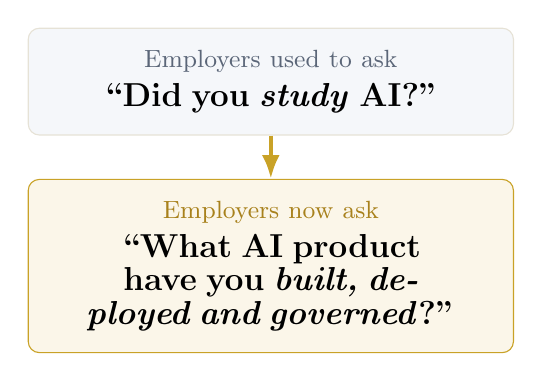
\begin{tikzpicture}
\node[draw=line,fill=rowbg,rounded corners=4pt,text width=5.6cm,align=center,inner sep=8pt] (a) {{\small\color{muted}Employers used to ask}\\[2pt]{\large\bfseries ``Did you \emph{study} AI?''}};
\node[draw=goldl,fill=goldbg,rounded corners=4pt,text width=5.6cm,align=center,inner sep=8pt,below=0.55cm of a] (b) {{\small\color{gold}Employers now ask}\\[2pt]{\large\bfseries ``What AI product have you \emph{built, deployed and governed}?''}};
\draw[-{Latex[length=3mm]},line width=1.5pt,goldl] (a) -- (b);
\end{tikzpicture}
\end{column}
\begin{column}{0.48\textwidth}
\small
\begin{itemize}\setlength\itemsep{6pt}
\item Every graduate in engineering, science and management will \textbf{work beside AI}; many will \textbf{build it}.
\item Universities that close the gap first lead in \textbf{placements, research, accreditation and rankings}.
\item This curriculum turns every unit into a \textbf{working artefact} and every course into a \textbf{deployable product}.
\item Aligned to \textbf{NEP 2020, OBE, NBA and NAAC} with CO--Bloom mapping.
\end{itemize}
\end{column}
\end{columns}
\end{frame}

\begin{frame}{The curriculum at a glance}\centering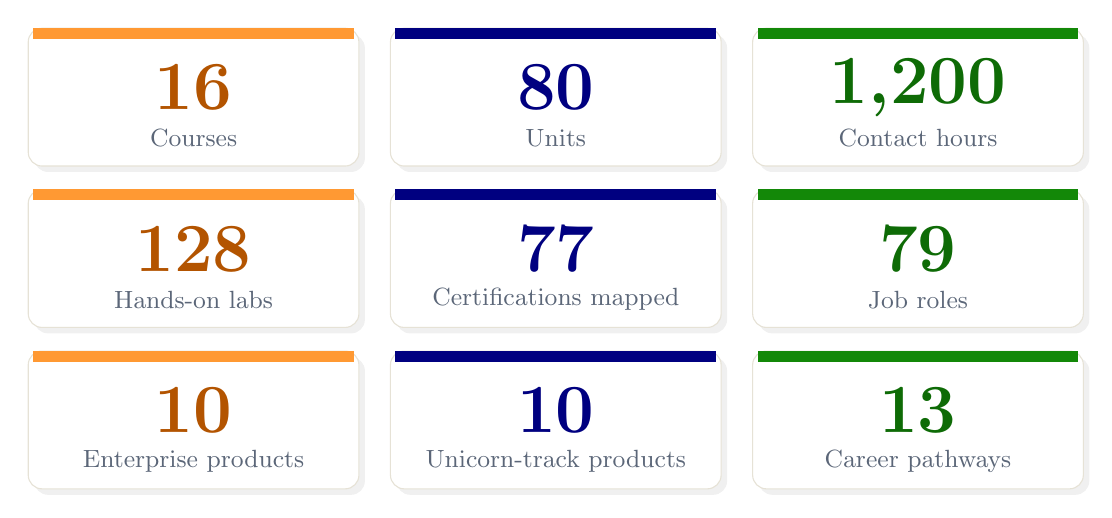
\begin{tikzpicture}
\node[draw=line,fill=white,rounded corners=5pt,minimum width=4.2cm,minimum height=1.75cm,drop shadow={opacity=0.12}] (s0) at (0.0,0.0) {};\fill[saffron] ([xshift=2pt]s0.north west) rectangle ([xshift=-2pt,yshift=-4pt]s0.north east);
\node[font=\fontsize{24}{26}\selectfont\bfseries,text=saffront] at ([yshift=0.12cm]s0.center) {16};\node[font=\small,text=muted] at ([yshift=-0.52cm]s0.center) {Courses};
\node[draw=line,fill=white,rounded corners=5pt,minimum width=4.2cm,minimum height=1.75cm,drop shadow={opacity=0.12}] (s1) at (4.6,0.0) {};\fill[chakra] ([xshift=2pt]s1.north west) rectangle ([xshift=-2pt,yshift=-4pt]s1.north east);
\node[font=\fontsize{24}{26}\selectfont\bfseries,text=chakra] at ([yshift=0.12cm]s1.center) {80};\node[font=\small,text=muted] at ([yshift=-0.52cm]s1.center) {Units};
\node[draw=line,fill=white,rounded corners=5pt,minimum width=4.2cm,minimum height=1.75cm,drop shadow={opacity=0.12}] (s2) at (9.2,0.0) {};\fill[igreen] ([xshift=2pt]s2.north west) rectangle ([xshift=-2pt,yshift=-4pt]s2.north east);
\node[font=\fontsize{24}{26}\selectfont\bfseries,text=igreent] at ([yshift=0.12cm]s2.center) {1,200};\node[font=\small,text=muted] at ([yshift=-0.52cm]s2.center) {Contact hours};
\node[draw=line,fill=white,rounded corners=5pt,minimum width=4.2cm,minimum height=1.75cm,drop shadow={opacity=0.12}] (s3) at (0.0,-2.05) {};\fill[saffron] ([xshift=2pt]s3.north west) rectangle ([xshift=-2pt,yshift=-4pt]s3.north east);
\node[font=\fontsize{24}{26}\selectfont\bfseries,text=saffront] at ([yshift=0.12cm]s3.center) {128};\node[font=\small,text=muted] at ([yshift=-0.52cm]s3.center) {Hands-on labs};
\node[draw=line,fill=white,rounded corners=5pt,minimum width=4.2cm,minimum height=1.75cm,drop shadow={opacity=0.12}] (s4) at (4.6,-2.05) {};\fill[chakra] ([xshift=2pt]s4.north west) rectangle ([xshift=-2pt,yshift=-4pt]s4.north east);
\node[font=\fontsize{24}{26}\selectfont\bfseries,text=chakra] at ([yshift=0.12cm]s4.center) {77};\node[font=\small,text=muted] at ([yshift=-0.52cm]s4.center) {Certifications mapped};
\node[draw=line,fill=white,rounded corners=5pt,minimum width=4.2cm,minimum height=1.75cm,drop shadow={opacity=0.12}] (s5) at (9.2,-2.05) {};\fill[igreen] ([xshift=2pt]s5.north west) rectangle ([xshift=-2pt,yshift=-4pt]s5.north east);
\node[font=\fontsize{24}{26}\selectfont\bfseries,text=igreent] at ([yshift=0.12cm]s5.center) {79};\node[font=\small,text=muted] at ([yshift=-0.52cm]s5.center) {Job roles};
\node[draw=line,fill=white,rounded corners=5pt,minimum width=4.2cm,minimum height=1.75cm,drop shadow={opacity=0.12}] (s6) at (0.0,-4.1) {};\fill[saffron] ([xshift=2pt]s6.north west) rectangle ([xshift=-2pt,yshift=-4pt]s6.north east);
\node[font=\fontsize{24}{26}\selectfont\bfseries,text=saffront] at ([yshift=0.12cm]s6.center) {10};\node[font=\small,text=muted] at ([yshift=-0.52cm]s6.center) {Enterprise products};
\node[draw=line,fill=white,rounded corners=5pt,minimum width=4.2cm,minimum height=1.75cm,drop shadow={opacity=0.12}] (s7) at (4.6,-4.1) {};\fill[chakra] ([xshift=2pt]s7.north west) rectangle ([xshift=-2pt,yshift=-4pt]s7.north east);
\node[font=\fontsize{24}{26}\selectfont\bfseries,text=chakra] at ([yshift=0.12cm]s7.center) {10};\node[font=\small,text=muted] at ([yshift=-0.52cm]s7.center) {Unicorn-track products};
\node[draw=line,fill=white,rounded corners=5pt,minimum width=4.2cm,minimum height=1.75cm,drop shadow={opacity=0.12}] (s8) at (9.2,-4.1) {};\fill[igreen] ([xshift=2pt]s8.north west) rectangle ([xshift=-2pt,yshift=-4pt]s8.north east);
\node[font=\fontsize{24}{26}\selectfont\bfseries,text=igreent] at ([yshift=0.12cm]s8.center) {13};\node[font=\small,text=muted] at ([yshift=-0.52cm]s8.center) {Career pathways};
\end{tikzpicture}\end{frame}
\begin{frame}{Three tracks, one product-engineering mindset}\centering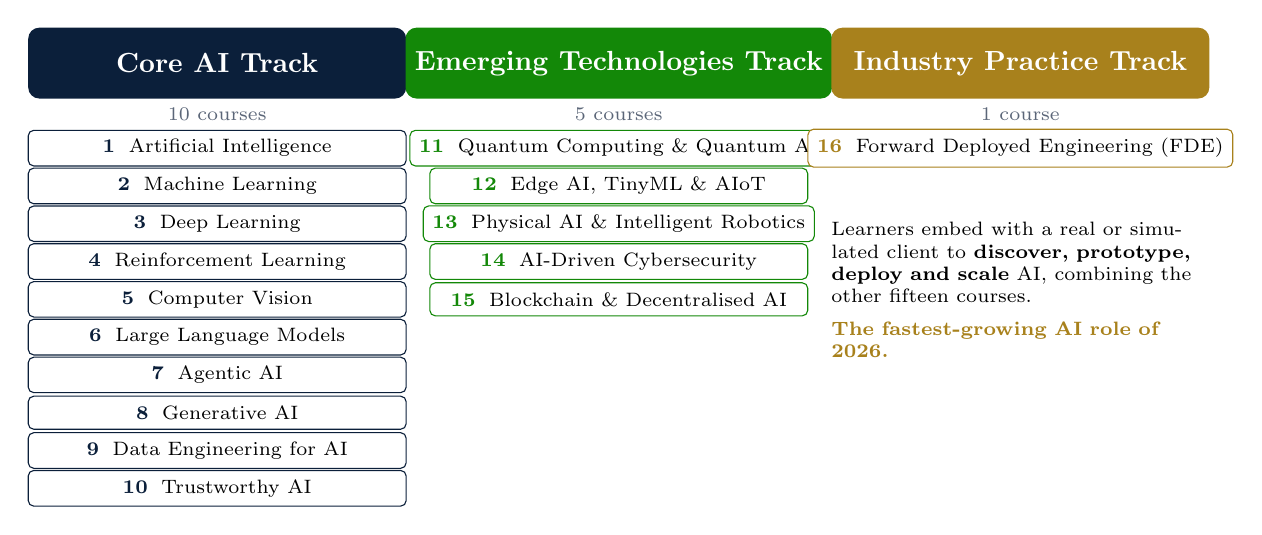
\begin{tikzpicture}
\node[fill=navy,rounded corners=4pt,minimum width=4.8cm,minimum height=0.9cm,text=white,font=\bfseries] at (0.0,0) {Core AI Track};
\node[font=\scriptsize\color{muted}] at (0.0,-0.65) {10 courses};
\node[draw=navy,fill=white,rounded corners=2pt,minimum width=4.8cm,minimum height=0.42cm,font=\scriptsize,anchor=center] at (0.0,-1.08) {\textbf{\color{navy}1}\; Artificial Intelligence};
\node[draw=navy,fill=white,rounded corners=2pt,minimum width=4.8cm,minimum height=0.42cm,font=\scriptsize,anchor=center] at (0.0,-1.56) {\textbf{\color{navy}2}\; Machine Learning};
\node[draw=navy,fill=white,rounded corners=2pt,minimum width=4.8cm,minimum height=0.42cm,font=\scriptsize,anchor=center] at (0.0,-2.04) {\textbf{\color{navy}3}\; Deep Learning};
\node[draw=navy,fill=white,rounded corners=2pt,minimum width=4.8cm,minimum height=0.42cm,font=\scriptsize,anchor=center] at (0.0,-2.52) {\textbf{\color{navy}4}\; Reinforcement Learning};
\node[draw=navy,fill=white,rounded corners=2pt,minimum width=4.8cm,minimum height=0.42cm,font=\scriptsize,anchor=center] at (0.0,-3.0) {\textbf{\color{navy}5}\; Computer Vision};
\node[draw=navy,fill=white,rounded corners=2pt,minimum width=4.8cm,minimum height=0.42cm,font=\scriptsize,anchor=center] at (0.0,-3.48) {\textbf{\color{navy}6}\; Large Language Models};
\node[draw=navy,fill=white,rounded corners=2pt,minimum width=4.8cm,minimum height=0.42cm,font=\scriptsize,anchor=center] at (0.0,-3.96) {\textbf{\color{navy}7}\; Agentic AI};
\node[draw=navy,fill=white,rounded corners=2pt,minimum width=4.8cm,minimum height=0.42cm,font=\scriptsize,anchor=center] at (0.0,-4.4399999999999995) {\textbf{\color{navy}8}\; Generative AI};
\node[draw=navy,fill=white,rounded corners=2pt,minimum width=4.8cm,minimum height=0.42cm,font=\scriptsize,anchor=center] at (0.0,-4.92) {\textbf{\color{navy}9}\; Data Engineering for AI};
\node[draw=navy,fill=white,rounded corners=2pt,minimum width=4.8cm,minimum height=0.42cm,font=\scriptsize,anchor=center] at (0.0,-5.4) {\textbf{\color{navy}10}\; Trustworthy AI};
\node[fill=igreen,rounded corners=4pt,minimum width=4.8cm,minimum height=0.9cm,text=white,font=\bfseries] at (5.1,0) {Emerging Technologies Track};
\node[font=\scriptsize\color{muted}] at (5.1,-0.65) {5 courses};
\node[draw=igreen,fill=white,rounded corners=2pt,minimum width=4.8cm,minimum height=0.42cm,font=\scriptsize,anchor=center] at (5.1,-1.08) {\textbf{\color{igreen}11}\; Quantum Computing \& Quantum AI};
\node[draw=igreen,fill=white,rounded corners=2pt,minimum width=4.8cm,minimum height=0.42cm,font=\scriptsize,anchor=center] at (5.1,-1.56) {\textbf{\color{igreen}12}\; Edge AI, TinyML \& AIoT};
\node[draw=igreen,fill=white,rounded corners=2pt,minimum width=4.8cm,minimum height=0.42cm,font=\scriptsize,anchor=center] at (5.1,-2.04) {\textbf{\color{igreen}13}\; Physical AI \& Intelligent Robotics};
\node[draw=igreen,fill=white,rounded corners=2pt,minimum width=4.8cm,minimum height=0.42cm,font=\scriptsize,anchor=center] at (5.1,-2.52) {\textbf{\color{igreen}14}\; AI-Driven Cybersecurity};
\node[draw=igreen,fill=white,rounded corners=2pt,minimum width=4.8cm,minimum height=0.42cm,font=\scriptsize,anchor=center] at (5.1,-3.0) {\textbf{\color{igreen}15}\; Blockchain \& Decentralised AI};
\node[fill=gold,rounded corners=4pt,minimum width=4.8cm,minimum height=0.9cm,text=white,font=\bfseries] at (10.2,0) {Industry Practice Track};
\node[font=\scriptsize\color{muted}] at (10.2,-0.65) {1 course};
\node[draw=gold,fill=white,rounded corners=2pt,minimum width=4.8cm,minimum height=0.42cm,font=\scriptsize,anchor=center] at (10.2,-1.08) {\textbf{\color{gold}16}\; Forward Deployed Engineering (FDE)};
\node[text width=4.8cm,font=\scriptsize,align=left,anchor=north] at (10.2,-1.9) {Learners embed with a real or simulated client to \textbf{discover, prototype, deploy and scale} AI, combining the other fifteen courses.\\[4pt]{\color{gold}\bfseries The fastest-growing AI role of 2026.}};
\end{tikzpicture}\end{frame}
\begin{frame}{Every course follows the same five-unit arc}\centering
\begin{tikzpicture}
\node[signal,signal to=east,fill=saffron,text=white,font=\small\bfseries,minimum height=1.3cm,minimum width=2.85cm,text width=2.3cm,align=center] at (0.0,0) {Unit I\\{\scriptsize Foundations}};
\node[signal,signal to=east,fill=goldl,text=white,font=\small\bfseries,minimum height=1.3cm,minimum width=2.85cm,text width=2.3cm,align=center] at (2.95,0) {Unit II\\{\scriptsize Core methods}};
\node[signal,signal to=east,fill=chakra,text=white,font=\small\bfseries,minimum height=1.3cm,minimum width=2.85cm,text width=2.3cm,align=center] at (5.9,0) {Unit III\\{\scriptsize Advanced methods}};
\node[signal,signal to=east,fill=navy2,text=white,font=\small\bfseries,minimum height=1.3cm,minimum width=2.85cm,text width=2.3cm,align=center] at (8.850000000000001,0) {Unit IV\\{\scriptsize Production engineering}};
\node[signal,signal to=east,fill=igreen,text=white,font=\small\bfseries,minimum height=1.3cm,minimum width=2.85cm,text width=2.3cm,align=center] at (11.8,0) {Unit V\\{\scriptsize Deploy \& capstone}};
\end{tikzpicture}\\[0.6cm]
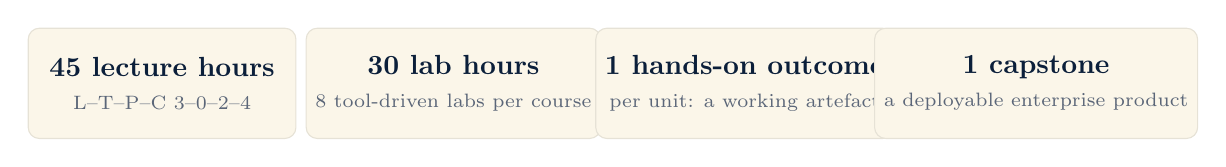
\begin{tikzpicture}
\foreach \x/\t/\d in {0/45 lecture hours/L--T--P--C 3--0--2--4, 3.7/30 lab hours/8 tool-driven labs per course, 7.4/1 hands-on outcome/per unit: a working artefact, 11.1/1 capstone/a deployable enterprise product}{
\node[draw=line,fill=goldbg,rounded corners=4pt,minimum width=3.4cm,minimum height=1.4cm,align=center] at (\x,0) {{\bfseries\color{navy}\t}\\{\scriptsize\color{muted}\d}};}
\end{tikzpicture}\\[0.4cm]
{\scriptsize\color{muted}Five course outcomes per course mapped to Bloom levels L2 Understand to L6 Create, ready for CO--PO--PSO attainment.}
\end{frame}
\begin{frame}{The 16 courses}\centering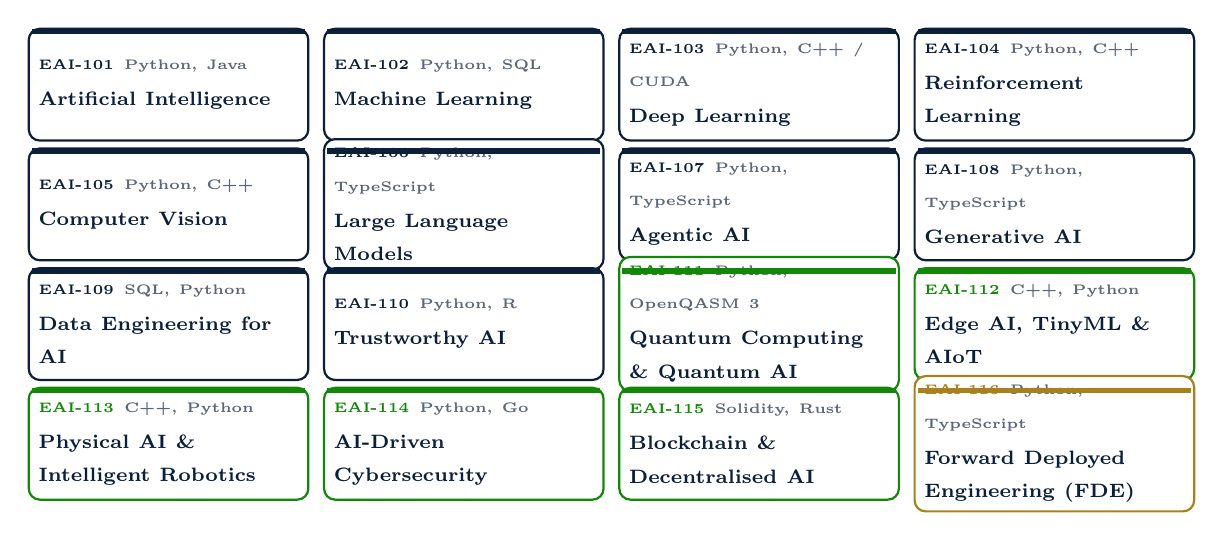
\begin{tikzpicture}
\node[draw=navy,line width=0.8pt,fill=white,rounded corners=4pt,minimum width=3.55cm,minimum height=1.42cm,text width=3.3cm,align=left] at (0.0,0.0) {\hyphenpenalty=10000\exhyphenpenalty=10000{\tiny\bfseries\color{navy}EAI-101\enspace\color{muted}Python, Java}\\[1pt]{\scriptsize\bfseries\color{navy} \mbox{Artificial} \mbox{Intelligence}}};
\fill[navy] (-1.7349999999999999,0.71) rectangle (1.7349999999999999,0.64);
\node[draw=navy,line width=0.8pt,fill=white,rounded corners=4pt,minimum width=3.55cm,minimum height=1.42cm,text width=3.3cm,align=left] at (3.75,0.0) {\hyphenpenalty=10000\exhyphenpenalty=10000{\tiny\bfseries\color{navy}EAI-102\enspace\color{muted}Python, SQL}\\[1pt]{\scriptsize\bfseries\color{navy} \mbox{Machine} \mbox{Learning}}};
\fill[navy] (2.015,0.71) rectangle (5.485,0.64);
\node[draw=navy,line width=0.8pt,fill=white,rounded corners=4pt,minimum width=3.55cm,minimum height=1.42cm,text width=3.3cm,align=left] at (7.5,0.0) {\hyphenpenalty=10000\exhyphenpenalty=10000{\tiny\bfseries\color{navy}EAI-103\enspace\color{muted}Python, C++ / CUDA}\\[1pt]{\scriptsize\bfseries\color{navy} \mbox{Deep} \mbox{Learning}}};
\fill[navy] (5.765,0.71) rectangle (9.235000000000001,0.64);
\node[draw=navy,line width=0.8pt,fill=white,rounded corners=4pt,minimum width=3.55cm,minimum height=1.42cm,text width=3.3cm,align=left] at (11.25,0.0) {\hyphenpenalty=10000\exhyphenpenalty=10000{\tiny\bfseries\color{navy}EAI-104\enspace\color{muted}Python, C++}\\[1pt]{\scriptsize\bfseries\color{navy} \mbox{Reinforcement} \mbox{Learning}}};
\fill[navy] (9.514999999999999,0.71) rectangle (12.985000000000001,0.64);
\node[draw=navy,line width=0.8pt,fill=white,rounded corners=4pt,minimum width=3.55cm,minimum height=1.42cm,text width=3.3cm,align=left] at (0.0,-1.52) {\hyphenpenalty=10000\exhyphenpenalty=10000{\tiny\bfseries\color{navy}EAI-105\enspace\color{muted}Python, C++}\\[1pt]{\scriptsize\bfseries\color{navy} \mbox{Computer} \mbox{Vision}}};
\fill[navy] (-1.7349999999999999,-0.81) rectangle (1.7349999999999999,-0.88);
\node[draw=navy,line width=0.8pt,fill=white,rounded corners=4pt,minimum width=3.55cm,minimum height=1.42cm,text width=3.3cm,align=left] at (3.75,-1.52) {\hyphenpenalty=10000\exhyphenpenalty=10000{\tiny\bfseries\color{navy}EAI-106\enspace\color{muted}Python, TypeScript}\\[1pt]{\scriptsize\bfseries\color{navy} \mbox{Large} \mbox{Language} \mbox{Models}}};
\fill[navy] (2.015,-0.81) rectangle (5.485,-0.88);
\node[draw=navy,line width=0.8pt,fill=white,rounded corners=4pt,minimum width=3.55cm,minimum height=1.42cm,text width=3.3cm,align=left] at (7.5,-1.52) {\hyphenpenalty=10000\exhyphenpenalty=10000{\tiny\bfseries\color{navy}EAI-107\enspace\color{muted}Python, TypeScript}\\[1pt]{\scriptsize\bfseries\color{navy} \mbox{Agentic} \mbox{AI}}};
\fill[navy] (5.765,-0.81) rectangle (9.235000000000001,-0.88);
\node[draw=navy,line width=0.8pt,fill=white,rounded corners=4pt,minimum width=3.55cm,minimum height=1.42cm,text width=3.3cm,align=left] at (11.25,-1.52) {\hyphenpenalty=10000\exhyphenpenalty=10000{\tiny\bfseries\color{navy}EAI-108\enspace\color{muted}Python, TypeScript}\\[1pt]{\scriptsize\bfseries\color{navy} \mbox{Generative} \mbox{AI}}};
\fill[navy] (9.514999999999999,-0.81) rectangle (12.985000000000001,-0.88);
\node[draw=navy,line width=0.8pt,fill=white,rounded corners=4pt,minimum width=3.55cm,minimum height=1.42cm,text width=3.3cm,align=left] at (0.0,-3.04) {\hyphenpenalty=10000\exhyphenpenalty=10000{\tiny\bfseries\color{navy}EAI-109\enspace\color{muted}SQL, Python}\\[1pt]{\scriptsize\bfseries\color{navy} \mbox{Data} \mbox{Engineering} \mbox{for} \mbox{AI}}};
\fill[navy] (-1.7349999999999999,-2.33) rectangle (1.7349999999999999,-2.4);
\node[draw=navy,line width=0.8pt,fill=white,rounded corners=4pt,minimum width=3.55cm,minimum height=1.42cm,text width=3.3cm,align=left] at (3.75,-3.04) {\hyphenpenalty=10000\exhyphenpenalty=10000{\tiny\bfseries\color{navy}EAI-110\enspace\color{muted}Python, R}\\[1pt]{\scriptsize\bfseries\color{navy} \mbox{Trustworthy} \mbox{AI}}};
\fill[navy] (2.015,-2.33) rectangle (5.485,-2.4);
\node[draw=igreen,line width=0.8pt,fill=white,rounded corners=4pt,minimum width=3.55cm,minimum height=1.42cm,text width=3.3cm,align=left] at (7.5,-3.04) {\hyphenpenalty=10000\exhyphenpenalty=10000{\tiny\bfseries\color{igreen}EAI-111\enspace\color{muted}Python, OpenQASM 3}\\[1pt]{\scriptsize\bfseries\color{navy} \mbox{Quantum} \mbox{Computing} \mbox{\&} \mbox{Quantum} \mbox{AI}}};
\fill[igreen] (5.765,-2.33) rectangle (9.235000000000001,-2.4);
\node[draw=igreen,line width=0.8pt,fill=white,rounded corners=4pt,minimum width=3.55cm,minimum height=1.42cm,text width=3.3cm,align=left] at (11.25,-3.04) {\hyphenpenalty=10000\exhyphenpenalty=10000{\tiny\bfseries\color{igreen}EAI-112\enspace\color{muted}C++, Python}\\[1pt]{\scriptsize\bfseries\color{navy} \mbox{Edge} \mbox{AI,} \mbox{TinyML} \mbox{\&} \mbox{AIoT}}};
\fill[igreen] (9.514999999999999,-2.33) rectangle (12.985000000000001,-2.4);
\node[draw=igreen,line width=0.8pt,fill=white,rounded corners=4pt,minimum width=3.55cm,minimum height=1.42cm,text width=3.3cm,align=left] at (0.0,-4.5600000000000005) {\hyphenpenalty=10000\exhyphenpenalty=10000{\tiny\bfseries\color{igreen}EAI-113\enspace\color{muted}C++, Python}\\[1pt]{\scriptsize\bfseries\color{navy} \mbox{Physical} \mbox{AI} \mbox{\&} \mbox{Intelligent} \mbox{Robotics}}};
\fill[igreen] (-1.7349999999999999,-3.8500000000000005) rectangle (1.7349999999999999,-3.9200000000000004);
\node[draw=igreen,line width=0.8pt,fill=white,rounded corners=4pt,minimum width=3.55cm,minimum height=1.42cm,text width=3.3cm,align=left] at (3.75,-4.5600000000000005) {\hyphenpenalty=10000\exhyphenpenalty=10000{\tiny\bfseries\color{igreen}EAI-114\enspace\color{muted}Python, Go}\\[1pt]{\scriptsize\bfseries\color{navy} \mbox{AI-Driven} \mbox{Cybersecurity}}};
\fill[igreen] (2.015,-3.8500000000000005) rectangle (5.485,-3.9200000000000004);
\node[draw=igreen,line width=0.8pt,fill=white,rounded corners=4pt,minimum width=3.55cm,minimum height=1.42cm,text width=3.3cm,align=left] at (7.5,-4.5600000000000005) {\hyphenpenalty=10000\exhyphenpenalty=10000{\tiny\bfseries\color{igreen}EAI-115\enspace\color{muted}Solidity, Rust}\\[1pt]{\scriptsize\bfseries\color{navy} \mbox{Blockchain} \mbox{\&} \mbox{Decentralised} \mbox{AI}}};
\fill[igreen] (5.765,-3.8500000000000005) rectangle (9.235000000000001,-3.9200000000000004);
\node[draw=gold,line width=0.8pt,fill=white,rounded corners=4pt,minimum width=3.55cm,minimum height=1.42cm,text width=3.3cm,align=left] at (11.25,-4.5600000000000005) {\hyphenpenalty=10000\exhyphenpenalty=10000{\tiny\bfseries\color{gold}EAI-116\enspace\color{muted}Python, TypeScript}\\[1pt]{\scriptsize\bfseries\color{navy} \mbox{Forward} \mbox{Deployed} \mbox{Engineering} \mbox{(FDE)}}};
\fill[gold] (9.514999999999999,-3.8500000000000005) rectangle (12.985000000000001,-3.9200000000000004);
\end{tikzpicture}\\[2pt]{\tiny\pill{navy}{Core AI} \pill{igreen}{Emerging Technologies} \pill{gold}{Industry Practice (FDE)} \quad\color{muted} Each tile shows the course code and its two main languages.}\end{frame}
\begin{frame}
\begin{tikzpicture}[remember picture,overlay]\fill[navy] ([yshift=-0.12cm]current page.north west) rectangle ([yshift=-1.55cm]current page.north east);
\node[anchor=west,text=white,align=left] at ([xshift=0.5cm,yshift=-0.85cm]current page.north west) {{\tiny\bfseries\color{goldl}COURSE 1 \,|\, EAI-101 \,|\, CORE AI TRACK}\\{\Large\bfseries Artificial Intelligence}\\[-1pt]{\scriptsize\itshape\color{white!85!navy}From search and reasoning to enterprise decision intelligence services}};\end{tikzpicture}
\vspace{0.72cm}
\begin{columns}[T]\begin{column}{0.53\textwidth}{\scriptsize\bfseries\color{gold}FIVE-UNIT CURRICULUM}\par\vspace{2pt}

\begin{tikzpicture}\node[fill=navy,text=white,font=\scriptsize\bfseries,minimum width=0.62cm,minimum height=0.62cm,rounded corners=2pt] (n) {I};\node[right=3pt of n.east,anchor=west,text width=7.1cm,font=\scriptsize,align=left] {\textbf{Foundations of Intelligent Systems}\\{\color{muted}Builds a simulated warehouse agent and an AI use-case canvas with KPIs and ROI estimate for a real business problem.}};\end{tikzpicture}\par\vspace{1pt}

\begin{tikzpicture}\node[fill=navy,text=white,font=\scriptsize\bfseries,minimum width=0.62cm,minimum height=0.62cm,rounded corners=2pt] (n) {II};\node[right=3pt of n.east,anchor=west,text width=7.1cm,font=\scriptsize,align=left] {\textbf{Search, Optimisation and Constraint Solving}\\{\color{muted}Delivers an A* route planner and an OR-Tools shift scheduler that beat a manual baseline on cost and time.}};\end{tikzpicture}\par\vspace{1pt}

\begin{tikzpicture}\node[fill=navy,text=white,font=\scriptsize\bfseries,minimum width=0.62cm,minimum height=0.62cm,rounded corners=2pt] (n) {III};\node[right=3pt of n.east,anchor=west,text width=7.1cm,font=\scriptsize,align=left] {\textbf{Knowledge Representation and Reasoning}\\{\color{muted}Creates a Neo4j product knowledge graph with Cypher queries and a rule engine that explains every inference.}};\end{tikzpicture}\par\vspace{1pt}

\begin{tikzpicture}\node[fill=navy,text=white,font=\scriptsize\bfseries,minimum width=0.62cm,minimum height=0.62cm,rounded corners=2pt] (n) {IV};\node[right=3pt of n.east,anchor=west,text width=7.1cm,font=\scriptsize,align=left] {\textbf{Uncertainty, Planning and Decision Making}\\{\color{muted}Builds a Bayesian loan-risk network and a PDDL planner that generates an automated IToperations runbook.}};\end{tikzpicture}\par\vspace{1pt}
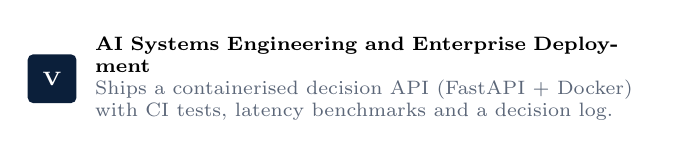
\begin{tikzpicture}\node[fill=navy,text=white,font=\scriptsize\bfseries,minimum width=0.62cm,minimum height=0.62cm,rounded corners=2pt] (n) {V};\node[right=3pt of n.east,anchor=west,text width=7.1cm,font=\scriptsize,align=left] {\textbf{AI Systems Engineering and Enterprise Deployment}\\{\color{muted}Ships a containerised decision API (FastAPI + Docker) with CI tests, latency benchmarks and a decision log.}};\end{tikzpicture}\par\vspace{1pt}
\vspace{2pt}
\begin{tikzpicture}\node[fill=goldbg,draw=goldl,rounded corners=3pt,text width=7.6cm,font=\scriptsize,align=left,inner sep=4pt] {{\bfseries\color{gold}Capstone:} \textbf{Enterprise Decision-Intelligence Engine}};\end{tikzpicture}
\end{column}\begin{column}{0.45\textwidth}{\scriptsize\bfseries\color{gold}SKILLS YOU WILL GAIN}\par\vspace{1pt}{\scriptsize\raggedright
\textcolor{saffron}{$\star$} Framing business problems as search, optimisation, planning or inference tasks\\
\textcolor{saffron}{$\star$} Pathfinding and heuristic search (A*, MCTS) for routing and games\\
\textcolor{saffron}{$\star$} Scheduling and resource allocation with OR-Tools, PuLP and constraint solvers\\
\textcolor{saffron}{$\star$} Building enterprise knowledge graphs in Neo4j with Cypher and SPARQL\\
\par}\vspace{4pt}{\scriptsize\bfseries\color{gold}JOBS}\par\vspace{1pt}{\scriptsize
\pill{saffron}{Fresher} \textbf{AI Engineer}\\[1pt]
\pill{saffron}{Fresher} \textbf{Decision Scientist}\\[1pt]
\pill{chakra}{Mid 3--5 yrs} \textbf{Optimisation Engineer}\\[1pt]
\pill{chakra}{Mid 3--5 yrs} \textbf{Knowledge Graph Engineer}\\[1pt]
}\vspace{3pt}{\scriptsize\bfseries\color{gold}INDICATIVE SALARY IN INDIA (₹ LPA)}\par\vspace{2pt}\begin{tikzpicture}
\node[fill=l1bg,minimum width=2.05cm,minimum height=0.95cm,rounded corners=2pt,align=center] (v0) at (0.0,0) {{\tiny\color{muted}Fresher}\\{\small\bfseries\color{saffront}₹6–15}};\fill[saffron] ([xshift=1pt]v0.north west) rectangle ([xshift=-1pt,yshift=-2.5pt]v0.north east);
\node[fill=l2bg,minimum width=2.05cm,minimum height=0.95cm,rounded corners=2pt,align=center] (v1) at (2.1,0) {{\tiny\color{muted}Mid}\\{\small\bfseries\color{chakra}₹15–30}};\fill[chakra] ([xshift=1pt]v1.north west) rectangle ([xshift=-1pt,yshift=-2.5pt]v1.north east);
\node[fill=l3bg,minimum width=2.05cm,minimum height=0.95cm,rounded corners=2pt,align=center] (v2) at (4.2,0) {{\tiny\color{muted}Senior}\\{\small\bfseries\color{igreent}₹30–60+}};\fill[igreen] ([xshift=1pt]v2.north west) rectangle ([xshift=-1pt,yshift=-2.5pt]v2.north east);
\end{tikzpicture}\par\vspace{2pt}{\tiny\color{muted}\textbf{Hiring:} Google, Microsoft, Amazon, Flipkart, Walmart Global Tech, JPMorgan Chase}
\end{column}\end{columns}\end{frame}
\begin{frame}
\begin{tikzpicture}[remember picture,overlay]\fill[navy] ([yshift=-0.12cm]current page.north west) rectangle ([yshift=-1.55cm]current page.north east);
\node[anchor=west,text=white,align=left] at ([xshift=0.5cm,yshift=-0.85cm]current page.north west) {{\tiny\bfseries\color{goldl}COURSE 2 \,|\, EAI-102 \,|\, CORE AI TRACK}\\{\Large\bfseries Machine Learning}\\[-1pt]{\scriptsize\itshape\color{white!85!navy}Building, validating and operating predictive models in production}};\end{tikzpicture}
\vspace{0.72cm}
\begin{columns}[T]\begin{column}{0.53\textwidth}{\scriptsize\bfseries\color{gold}FIVE-UNIT CURRICULUM}\par\vspace{2pt}

\begin{tikzpicture}\node[fill=navy,text=white,font=\scriptsize\bfseries,minimum width=0.62cm,minimum height=0.62cm,rounded corners=2pt] (n) {I};\node[right=3pt of n.east,anchor=west,text width=7.1cm,font=\scriptsize,align=left] {\textbf{ML Foundations and Problem Framing}\\{\color{muted}Produces an EDA and data-quality report and a baseline model with a documented KPI-to-metric mapping.}};\end{tikzpicture}\par\vspace{1pt}

\begin{tikzpicture}\node[fill=navy,text=white,font=\scriptsize\bfseries,minimum width=0.62cm,minimum height=0.62cm,rounded corners=2pt] (n) {II};\node[right=3pt of n.east,anchor=west,text width=7.1cm,font=\scriptsize,align=left] {\textbf{Supervised Learning}\\{\color{muted}Trains a calibrated credit-scoring model and a gradient-boosted churn model that outperform baselines.}};\end{tikzpicture}\par\vspace{1pt}

\begin{tikzpicture}\node[fill=navy,text=white,font=\scriptsize\bfseries,minimum width=0.62cm,minimum height=0.62cm,rounded corners=2pt] (n) {III};\node[right=3pt of n.east,anchor=west,text width=7.1cm,font=\scriptsize,align=left] {\textbf{Unsupervised Learning and Representation}\\{\color{muted}Delivers customer segments with UMAP visualisation, an anomaly detector and a working recommender.}};\end{tikzpicture}\par\vspace{1pt}

\begin{tikzpicture}\node[fill=navy,text=white,font=\scriptsize\bfseries,minimum width=0.62cm,minimum height=0.62cm,rounded corners=2pt] (n) {IV};\node[right=3pt of n.east,anchor=west,text width=7.1cm,font=\scriptsize,align=left] {\textbf{Model Evaluation, Tuning and Interpretability}\\{\color{muted}Produces an Optuna-tuned model with leakage checks, cost-curve analysis and a SHAP explanation report.}};\end{tikzpicture}\par\vspace{1pt}

\begin{tikzpicture}\node[fill=navy,text=white,font=\scriptsize\bfseries,minimum width=0.62cm,minimum height=0.62cm,rounded corners=2pt] (n) {V};\node[right=3pt of n.east,anchor=west,text width=7.1cm,font=\scriptsize,align=left] {\textbf{MLOps and Enterprise Deployment}\\{\color{muted}Deploys an MLflow-tracked model via BentoML with Evidently drift alerts and an automated retraining trigger.}};\end{tikzpicture}\par\vspace{1pt}
\vspace{2pt}
\begin{tikzpicture}\node[fill=goldbg,draw=goldl,rounded corners=3pt,text width=7.6cm,font=\scriptsize,align=left,inner sep=4pt] {{\bfseries\color{gold}Capstone:} \textbf{Customer Intelligence Platform}};\end{tikzpicture}
\end{column}\begin{column}{0.45\textwidth}{\scriptsize\bfseries\color{gold}SKILLS YOU WILL GAIN}\par\vspace{1pt}{\scriptsize\raggedright
\textcolor{saffron}{$\star$} Translating business KPIs into ML targets, labels and metrics\\
\textcolor{saffron}{$\star$} Feature engineering and data preparation with pandas and scikit-learn\\
\textcolor{saffron}{$\star$} Gradient-boosted models (XGBoost, LightGBM) for tabular data\\
\textcolor{saffron}{$\star$} Clustering, dimensionality reduction and anomaly detection\\
\par}\vspace{4pt}{\scriptsize\bfseries\color{gold}JOBS}\par\vspace{1pt}{\scriptsize
\pill{saffron}{Fresher} \textbf{Data Scientist}\\[1pt]
\pill{saffron}{Fresher} \textbf{Machine Learning Engineer}\\[1pt]
\pill{saffron}{Fresher} \textbf{Analytics Engineer}\\[1pt]
\pill{chakra}{Mid 3--5 yrs} \textbf{MLOps Engineer}\\[1pt]
}\vspace{3pt}{\scriptsize\bfseries\color{gold}INDICATIVE SALARY IN INDIA (₹ LPA)}\par\vspace{2pt}\begin{tikzpicture}
\node[fill=l1bg,minimum width=2.05cm,minimum height=0.95cm,rounded corners=2pt,align=center] (v0) at (0.0,0) {{\tiny\color{muted}Fresher}\\{\small\bfseries\color{saffront}₹5–12}};\fill[saffron] ([xshift=1pt]v0.north west) rectangle ([xshift=-1pt,yshift=-2.5pt]v0.north east);
\node[fill=l2bg,minimum width=2.05cm,minimum height=0.95cm,rounded corners=2pt,align=center] (v1) at (2.1,0) {{\tiny\color{muted}Mid}\\{\small\bfseries\color{chakra}₹18–35}};\fill[chakra] ([xshift=1pt]v1.north west) rectangle ([xshift=-1pt,yshift=-2.5pt]v1.north east);
\node[fill=l3bg,minimum width=2.05cm,minimum height=0.95cm,rounded corners=2pt,align=center] (v2) at (4.2,0) {{\tiny\color{muted}Senior}\\{\small\bfseries\color{igreent}₹35–65+}};\fill[igreen] ([xshift=1pt]v2.north west) rectangle ([xshift=-1pt,yshift=-2.5pt]v2.north east);
\end{tikzpicture}\par\vspace{2pt}{\tiny\color{muted}\textbf{Hiring:} Google, Amazon, Microsoft, Flipkart, PhonePe, Razorpay}
\end{column}\end{columns}\end{frame}
\begin{frame}
\begin{tikzpicture}[remember picture,overlay]\fill[navy] ([yshift=-0.12cm]current page.north west) rectangle ([yshift=-1.55cm]current page.north east);
\node[anchor=west,text=white,align=left] at ([xshift=0.5cm,yshift=-0.85cm]current page.north west) {{\tiny\bfseries\color{goldl}COURSE 3 \,|\, EAI-103 \,|\, CORE AI TRACK}\\{\Large\bfseries Deep Learning}\\[-1pt]{\scriptsize\itshape\color{white!85!navy}Neural architectures engineered for accuracy, scale and efficient inference}};\end{tikzpicture}
\vspace{0.72cm}
\begin{columns}[T]\begin{column}{0.53\textwidth}{\scriptsize\bfseries\color{gold}FIVE-UNIT CURRICULUM}\par\vspace{2pt}

\begin{tikzpicture}\node[fill=navy,text=white,font=\scriptsize\bfseries,minimum width=0.62cm,minimum height=0.62cm,rounded corners=2pt] (n) {I};\node[right=3pt of n.east,anchor=west,text width=7.1cm,font=\scriptsize,align=left] {\textbf{Neural Network Foundations}\\{\color{muted}Implements an MLP from scratch with autograd on GPU and verifies gradients against PyTorch.}};\end{tikzpicture}\par\vspace{1pt}

\begin{tikzpicture}\node[fill=navy,text=white,font=\scriptsize\bfseries,minimum width=0.62cm,minimum height=0.62cm,rounded corners=2pt] (n) {II};\node[right=3pt of n.east,anchor=west,text width=7.1cm,font=\scriptsize,align=left] {\textbf{Optimisation and Regularisation}\\{\color{muted}Produces an optimiser/LR-schedule comparison study and a debugged, stable training recipe.}};\end{tikzpicture}\par\vspace{1pt}

\begin{tikzpicture}\node[fill=navy,text=white,font=\scriptsize\bfseries,minimum width=0.62cm,minimum height=0.62cm,rounded corners=2pt] (n) {III};\node[right=3pt of n.east,anchor=west,text width=7.1cm,font=\scriptsize,align=left] {\textbf{Convolutional and Sequence Architectures}\\{\color{muted}Fine-tunes a ResNet product classifier and an LSTM sensor forecaster with reported accuracy and error.}};\end{tikzpicture}\par\vspace{1pt}

\begin{tikzpicture}\node[fill=navy,text=white,font=\scriptsize\bfseries,minimum width=0.62cm,minimum height=0.62cm,rounded corners=2pt] (n) {IV};\node[right=3pt of n.east,anchor=west,text width=7.1cm,font=\scriptsize,align=left] {\textbf{Attention, Transformers and Graph Networks}\\{\color{muted}Fine-tunes a Transformer text classifier and trains a GNN fraud detector on a transaction graph.}};\end{tikzpicture}\par\vspace{1pt}
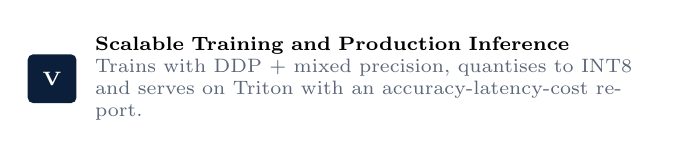
\begin{tikzpicture}\node[fill=navy,text=white,font=\scriptsize\bfseries,minimum width=0.62cm,minimum height=0.62cm,rounded corners=2pt] (n) {V};\node[right=3pt of n.east,anchor=west,text width=7.1cm,font=\scriptsize,align=left] {\textbf{Scalable Training and Production Inference}\\{\color{muted}Trains with DDP + mixed precision, quantises to INT8 and serves on Triton with an accuracy-latency-cost report.}};\end{tikzpicture}\par\vspace{1pt}
\vspace{2pt}
\begin{tikzpicture}\node[fill=goldbg,draw=goldl,rounded corners=3pt,text width=7.6cm,font=\scriptsize,align=left,inner sep=4pt] {{\bfseries\color{gold}Capstone:} \textbf{Deep Learning Inference Service}};\end{tikzpicture}
\end{column}\begin{column}{0.45\textwidth}{\scriptsize\bfseries\color{gold}SKILLS YOU WILL GAIN}\par\vspace{1pt}{\scriptsize\raggedright
\textcolor{saffron}{$\star$} Building and training neural networks in PyTorch from first principles\\
\textcolor{saffron}{$\star$} Optimisers, regularisation and training stability\\
\textcolor{saffron}{$\star$} CNNs, RNNs/LSTMs and sequence modelling\\
\textcolor{saffron}{$\star$} Transformers, attention and graph neural networks\\
\par}\vspace{4pt}{\scriptsize\bfseries\color{gold}JOBS}\par\vspace{1pt}{\scriptsize
\pill{saffron}{Fresher} \textbf{Deep Learning Engineer}\\[1pt]
\pill{chakra}{Mid 3--5 yrs} \textbf{AI Research Engineer}\\[1pt]
\pill{chakra}{Mid 3--5 yrs} \textbf{ML Performance Engineer}\\[1pt]
\pill{chakra}{Mid 3--5 yrs} \textbf{Edge AI Engineer}\\[1pt]
}\vspace{3pt}{\scriptsize\bfseries\color{gold}INDICATIVE SALARY IN INDIA (₹ LPA)}\par\vspace{2pt}\begin{tikzpicture}
\node[fill=l1bg,minimum width=2.05cm,minimum height=0.95cm,rounded corners=2pt,align=center] (v0) at (0.0,0) {{\tiny\color{muted}Fresher}\\{\small\bfseries\color{saffront}₹6–15}};\fill[saffron] ([xshift=1pt]v0.north west) rectangle ([xshift=-1pt,yshift=-2.5pt]v0.north east);
\node[fill=l2bg,minimum width=2.05cm,minimum height=0.95cm,rounded corners=2pt,align=center] (v1) at (2.1,0) {{\tiny\color{muted}Mid}\\{\small\bfseries\color{chakra}₹18–35}};\fill[chakra] ([xshift=1pt]v1.north west) rectangle ([xshift=-1pt,yshift=-2.5pt]v1.north east);
\node[fill=l3bg,minimum width=2.05cm,minimum height=0.95cm,rounded corners=2pt,align=center] (v2) at (4.2,0) {{\tiny\color{muted}Senior}\\{\small\bfseries\color{igreent}₹35–70+}};\fill[igreen] ([xshift=1pt]v2.north west) rectangle ([xshift=-1pt,yshift=-2.5pt]v2.north east);
\end{tikzpicture}\par\vspace{2pt}{\tiny\color{muted}\textbf{Hiring:} NVIDIA, Google, Microsoft, Qualcomm, Intel, Samsung R\&D}
\end{column}\end{columns}\end{frame}
\begin{frame}
\begin{tikzpicture}[remember picture,overlay]\fill[navy] ([yshift=-0.12cm]current page.north west) rectangle ([yshift=-1.55cm]current page.north east);
\node[anchor=west,text=white,align=left] at ([xshift=0.5cm,yshift=-0.85cm]current page.north west) {{\tiny\bfseries\color{goldl}COURSE 4 \,|\, EAI-104 \,|\, CORE AI TRACK}\\{\Large\bfseries Reinforcement Learning}\\[-1pt]{\scriptsize\itshape\color{white!85!navy}Sequential decision-making for optimisation, control and AI alignment}};\end{tikzpicture}
\vspace{0.72cm}
\begin{columns}[T]\begin{column}{0.53\textwidth}{\scriptsize\bfseries\color{gold}FIVE-UNIT CURRICULUM}\par\vspace{2pt}

\begin{tikzpicture}\node[fill=navy,text=white,font=\scriptsize\bfseries,minimum width=0.62cm,minimum height=0.62cm,rounded corners=2pt] (n) {I};\node[right=3pt of n.east,anchor=west,text width=7.1cm,font=\scriptsize,align=left] {\textbf{RL Foundations and MDPs}\\{\color{muted}Solves an inventory MDP with value iteration and deploys a contextual bandit for offer recommendation.}};\end{tikzpicture}\par\vspace{1pt}

\begin{tikzpicture}\node[fill=navy,text=white,font=\scriptsize\bfseries,minimum width=0.62cm,minimum height=0.62cm,rounded corners=2pt] (n) {II};\node[right=3pt of n.east,anchor=west,text width=7.1cm,font=\scriptsize,align=left] {\textbf{Model-Free Tabular Methods}\\{\color{muted}Builds a custom Gymnasium environment and a Q-learning agent with a shaped reward function.}};\end{tikzpicture}\par\vspace{1pt}

\begin{tikzpicture}\node[fill=navy,text=white,font=\scriptsize\bfseries,minimum width=0.62cm,minimum height=0.62cm,rounded corners=2pt] (n) {III};\node[right=3pt of n.east,anchor=west,text width=7.1cm,font=\scriptsize,align=left] {\textbf{Deep Reinforcement Learning}\\{\color{muted}Trains DQN and PPO agents and compares sample efficiency and stability on standard benchmarks.}};\end{tikzpicture}\par\vspace{1pt}

\begin{tikzpicture}\node[fill=navy,text=white,font=\scriptsize\bfseries,minimum width=0.62cm,minimum height=0.62cm,rounded corners=2pt] (n) {IV};\node[right=3pt of n.east,anchor=west,text width=7.1cm,font=\scriptsize,align=left] {\textbf{Advanced and Offline RL}\\{\color{muted}Trains an offline RL policy on logged data and evaluates it with off-policy estimators before deployment.}};\end{tikzpicture}\par\vspace{1pt}

\begin{tikzpicture}\node[fill=navy,text=white,font=\scriptsize\bfseries,minimum width=0.62cm,minimum height=0.62cm,rounded corners=2pt] (n) {V};\node[right=3pt of n.east,anchor=west,text width=7.1cm,font=\scriptsize,align=left] {\textbf{RL for Enterprise and LLM Alignment}\\{\color{muted}Aligns a small LLM with a reward model + DPO and runs a pricing policy in shadow mode with guardrails.}};\end{tikzpicture}\par\vspace{1pt}
\vspace{2pt}
\begin{tikzpicture}\node[fill=goldbg,draw=goldl,rounded corners=3pt,text width=7.6cm,font=\scriptsize,align=left,inner sep=4pt] {{\bfseries\color{gold}Capstone:} \textbf{Adaptive Pricing and Inventory Optimiser}};\end{tikzpicture}
\end{column}\begin{column}{0.45\textwidth}{\scriptsize\bfseries\color{gold}SKILLS YOU WILL GAIN}\par\vspace{1pt}{\scriptsize\raggedright
\textcolor{saffron}{$\star$} Modelling sequential decisions as Markov decision processes\\
\textcolor{saffron}{$\star$} Dynamic programming, Q-learning and SARSA\\
\textcolor{saffron}{$\star$} Deep RL: DQN, PPO and actor-critic methods\\
\textcolor{saffron}{$\star$} Reward design, exploration and training stability\\
\par}\vspace{4pt}{\scriptsize\bfseries\color{gold}JOBS}\par\vspace{1pt}{\scriptsize
\pill{saffron}{Fresher} \textbf{Reinforcement Learning Engineer}\\[1pt]
\pill{saffron}{Fresher} \textbf{Decision Scientist}\\[1pt]
\pill{chakra}{Mid 3--5 yrs} \textbf{Robotics AI Engineer}\\[1pt]
\pill{chakra}{Mid 3--5 yrs} \textbf{LLM Alignment Engineer}\\[1pt]
}\vspace{3pt}{\scriptsize\bfseries\color{gold}INDICATIVE SALARY IN INDIA (₹ LPA)}\par\vspace{2pt}\begin{tikzpicture}
\node[fill=l1bg,minimum width=2.05cm,minimum height=0.95cm,rounded corners=2pt,align=center] (v0) at (0.0,0) {{\tiny\color{muted}Fresher}\\{\small\bfseries\color{saffront}₹6–15}};\fill[saffron] ([xshift=1pt]v0.north west) rectangle ([xshift=-1pt,yshift=-2.5pt]v0.north east);
\node[fill=l2bg,minimum width=2.05cm,minimum height=0.95cm,rounded corners=2pt,align=center] (v1) at (2.1,0) {{\tiny\color{muted}Mid}\\{\small\bfseries\color{chakra}₹18–40}};\fill[chakra] ([xshift=1pt]v1.north west) rectangle ([xshift=-1pt,yshift=-2.5pt]v1.north east);
\node[fill=l3bg,minimum width=2.05cm,minimum height=0.95cm,rounded corners=2pt,align=center] (v2) at (4.2,0) {{\tiny\color{muted}Senior}\\{\small\bfseries\color{igreent}₹40–70+}};\fill[igreen] ([xshift=1pt]v2.north west) rectangle ([xshift=-1pt,yshift=-2.5pt]v2.north east);
\end{tikzpicture}\par\vspace{2pt}{\tiny\color{muted}\textbf{Hiring:} Google DeepMind, Microsoft Research India, Amazon, Uber, Flipkart, Dream11}
\end{column}\end{columns}\end{frame}
\begin{frame}
\begin{tikzpicture}[remember picture,overlay]\fill[navy] ([yshift=-0.12cm]current page.north west) rectangle ([yshift=-1.55cm]current page.north east);
\node[anchor=west,text=white,align=left] at ([xshift=0.5cm,yshift=-0.85cm]current page.north west) {{\tiny\bfseries\color{goldl}COURSE 5 \,|\, EAI-105 \,|\, CORE AI TRACK}\\{\Large\bfseries Computer Vision}\\[-1pt]{\scriptsize\itshape\color{white!85!navy}Visual perception products for inspection, documents, retail and video analytics}};\end{tikzpicture}
\vspace{0.72cm}
\begin{columns}[T]\begin{column}{0.53\textwidth}{\scriptsize\bfseries\color{gold}FIVE-UNIT CURRICULUM}\par\vspace{2pt}

\begin{tikzpicture}\node[fill=navy,text=white,font=\scriptsize\bfseries,minimum width=0.62cm,minimum height=0.62cm,rounded corners=2pt] (n) {I};\node[right=3pt of n.east,anchor=west,text width=7.1cm,font=\scriptsize,align=left] {\textbf{Image Formation and Classical Vision}\\{\color{muted}Calibrates a camera and builds a measurement/stitching tool using classical features and homography.}};\end{tikzpicture}\par\vspace{1pt}

\begin{tikzpicture}\node[fill=navy,text=white,font=\scriptsize\bfseries,minimum width=0.62cm,minimum height=0.62cm,rounded corners=2pt] (n) {II};\node[right=3pt of n.east,anchor=west,text width=7.1cm,font=\scriptsize,align=left] {\textbf{Deep Image Classification and Representation}\\{\color{muted}Delivers a defect classifier via transfer learning and a visual-search service using embeddings.}};\end{tikzpicture}\par\vspace{1pt}

\begin{tikzpicture}\node[fill=navy,text=white,font=\scriptsize\bfseries,minimum width=0.62cm,minimum height=0.62cm,rounded corners=2pt] (n) {III};\node[right=3pt of n.east,anchor=west,text width=7.1cm,font=\scriptsize,align=left] {\textbf{Detection, Segmentation and Tracking}\\{\color{muted}Trains a YOLO detector and SAM-assisted segmentation on custom data and a people-counting tracker (mAP, MOTA reported).}};\end{tikzpicture}\par\vspace{1pt}

\begin{tikzpicture}\node[fill=navy,text=white,font=\scriptsize\bfseries,minimum width=0.62cm,minimum height=0.62cm,rounded corners=2pt] (n) {IV};\node[right=3pt of n.east,anchor=west,text width=7.1cm,font=\scriptsize,align=left] {\textbf{3D, Video and Vision–Language Models}\\{\color{muted}Builds an invoice OCR + key-field extraction pipeline and a zero-shot CLIP/VLM classification demo.}};\end{tikzpicture}\par\vspace{1pt}

\begin{tikzpicture}\node[fill=navy,text=white,font=\scriptsize\bfseries,minimum width=0.62cm,minimum height=0.62cm,rounded corners=2pt] (n) {V};\node[right=3pt of n.east,anchor=west,text width=7.1cm,font=\scriptsize,align=left] {\textbf{Edge Deployment and Vision Product Engineering}\\{\color{muted}Deploys a real-time RTSP vision pipeline on Jetson with TensorRT, face blurring and an events dashboard.}};\end{tikzpicture}\par\vspace{1pt}
\vspace{2pt}
\begin{tikzpicture}\node[fill=goldbg,draw=goldl,rounded corners=3pt,text width=7.6cm,font=\scriptsize,align=left,inner sep=4pt] {{\bfseries\color{gold}Capstone:} \textbf{Smart Visual Inspection System}};\end{tikzpicture}
\end{column}\begin{column}{0.45\textwidth}{\scriptsize\bfseries\color{gold}SKILLS YOU WILL GAIN}\par\vspace{1pt}{\scriptsize\raggedright
\textcolor{saffron}{$\star$} Image processing, camera calibration and geometric vision with OpenCV\\
\textcolor{saffron}{$\star$} Image classification and transfer learning\\
\textcolor{saffron}{$\star$} Object detection, segmentation and multi-object tracking (YOLO-class models)\\
\textcolor{saffron}{$\star$} Document AI: OCR and layout understanding\\
\par}\vspace{4pt}{\scriptsize\bfseries\color{gold}JOBS}\par\vspace{1pt}{\scriptsize
\pill{saffron}{Fresher} \textbf{Computer Vision Engineer}\\[1pt]
\pill{saffron}{Fresher} \textbf{Document AI Engineer}\\[1pt]
\pill{chakra}{Mid 3--5 yrs} \textbf{Video Analytics Engineer}\\[1pt]
\pill{chakra}{Mid 3--5 yrs} \textbf{Edge AI Engineer}\\[1pt]
}\vspace{3pt}{\scriptsize\bfseries\color{gold}INDICATIVE SALARY IN INDIA (₹ LPA)}\par\vspace{2pt}\begin{tikzpicture}
\node[fill=l1bg,minimum width=2.05cm,minimum height=0.95cm,rounded corners=2pt,align=center] (v0) at (0.0,0) {{\tiny\color{muted}Fresher}\\{\small\bfseries\color{saffront}₹8–16}};\fill[saffron] ([xshift=1pt]v0.north west) rectangle ([xshift=-1pt,yshift=-2.5pt]v0.north east);
\node[fill=l2bg,minimum width=2.05cm,minimum height=0.95cm,rounded corners=2pt,align=center] (v1) at (2.1,0) {{\tiny\color{muted}Mid}\\{\small\bfseries\color{chakra}₹15–30}};\fill[chakra] ([xshift=1pt]v1.north west) rectangle ([xshift=-1pt,yshift=-2.5pt]v1.north east);
\node[fill=l3bg,minimum width=2.05cm,minimum height=0.95cm,rounded corners=2pt,align=center] (v2) at (4.2,0) {{\tiny\color{muted}Senior}\\{\small\bfseries\color{igreent}₹26–70}};\fill[igreen] ([xshift=1pt]v2.north west) rectangle ([xshift=-1pt,yshift=-2.5pt]v2.north east);
\end{tikzpicture}\par\vspace{2pt}{\tiny\color{muted}\textbf{Hiring:} NVIDIA, Qualcomm, Intel, Samsung R\&D, Bosch, Continental}
\end{column}\end{columns}\end{frame}
\begin{frame}
\begin{tikzpicture}[remember picture,overlay]\fill[navy] ([yshift=-0.12cm]current page.north west) rectangle ([yshift=-1.55cm]current page.north east);
\node[anchor=west,text=white,align=left] at ([xshift=0.5cm,yshift=-0.85cm]current page.north west) {{\tiny\bfseries\color{goldl}COURSE 6 \,|\, EAI-106 \,|\, CORE AI TRACK}\\{\Large\bfseries Large Language Models}\\[-1pt]{\scriptsize\itshape\color{white!85!navy}Pre-training, adaptation, retrieval grounding and LLMOps for enterprise language services}};\end{tikzpicture}
\vspace{0.72cm}
\begin{columns}[T]\begin{column}{0.53\textwidth}{\scriptsize\bfseries\color{gold}FIVE-UNIT CURRICULUM}\par\vspace{2pt}

\begin{tikzpicture}\node[fill=navy,text=white,font=\scriptsize\bfseries,minimum width=0.62cm,minimum height=0.62cm,rounded corners=2pt] (n) {I};\node[right=3pt of n.east,anchor=west,text width=7.1cm,font=\scriptsize,align=left] {\textbf{Language Modelling Foundations}\\{\color{muted}Trains a BPE tokeniser and a mini-GPT from scratch and measures perplexity and KV-cache speed-up.}};\end{tikzpicture}\par\vspace{1pt}
\begin{tikzpicture}\node[fill=navy,text=white,font=\scriptsize\bfseries,minimum width=0.62cm,minimum height=0.62cm,rounded corners=2pt] (n) {II};\node[right=3pt of n.east,anchor=west,text width=7.1cm,font=\scriptsize,align=left] {\textbf{Prompting, Reasoning and Structured Output}\\{\color{muted}Builds a versioned prompt library with JSON-schema outputs and an automated prompt regression test suite.}};\end{tikzpicture}\par\vspace{1pt}
\begin{tikzpicture}\node[fill=navy,text=white,font=\scriptsize\bfseries,minimum width=0.62cm,minimum height=0.62cm,rounded corners=2pt] (n) {III};\node[right=3pt of n.east,anchor=west,text width=7.1cm,font=\scriptsize,align=left] {\textbf{Fine-Tuning and Alignment}\\{\color{muted}Fine-tunes a 7-8B model with QLoRA and aligns it with DPO, with before/after evaluation.}};\end{tikzpicture}\par\vspace{1pt}
\begin{tikzpicture}\node[fill=navy,text=white,font=\scriptsize\bfseries,minimum width=0.62cm,minimum height=0.62cm,rounded corners=2pt] (n) {IV};\node[right=3pt of n.east,anchor=west,text width=7.1cm,font=\scriptsize,align=left] {\textbf{Retrieval-Augmented Generation}\\{\color{muted}Delivers a hybrid-search RAG assistant with re-ranking, citations and permission-aware retrieval.}};\end{tikzpicture}\par\vspace{1pt}
\begin{tikzpicture}\node[fill=navy,text=white,font=\scriptsize\bfseries,minimum width=0.62cm,minimum height=0.62cm,rounded corners=2pt] (n) {V};\node[right=3pt of n.east,anchor=west,text width=7.1cm,font=\scriptsize,align=left] {\textbf{LLMOps, Evaluation and Production Serving}\\{\color{muted}Serves a quantised model on vLLM behind a gateway with RAGAS evaluation, tracing and token-cost dashboards.}};\end{tikzpicture}\par\vspace{1pt}
\vspace{2pt}\begin{tikzpicture}\node[fill=goldbg,draw=goldl,rounded corners=3pt,text width=7.6cm,font=\scriptsize,align=left,inner sep=4pt] {{\bfseries\color{gold}Capstone:} \textbf{Enterprise Knowledge Assistant}};\end{tikzpicture}
\end{column}\begin{column}{0.45\textwidth}{\scriptsize\bfseries\color{gold}SKILLS YOU WILL GAIN}\par\vspace{1pt}{\scriptsize\raggedright
\textcolor{saffron}{$\star$} How transformers and tokenisers work inside an LLM\\
\textcolor{saffron}{$\star$} Prompt engineering, reasoning patterns and structured (JSON) outputs\\
\textcolor{saffron}{$\star$} Fine-tuning with LoRA/QLoRA on domain data\\
\textcolor{saffron}{$\star$} Retrieval-augmented generation with embeddings and vector databases\\
\par}\vspace{4pt}{\scriptsize\bfseries\color{gold}JOBS}\par\vspace{1pt}{\scriptsize
\pill{saffron}{Fresher} \textbf{LLM Engineer}\\[1pt]
\pill{saffron}{Fresher} \textbf{AI Engineer (GenAI)}\\[1pt]
\pill{saffron}{Fresher} \textbf{NLP Engineer}\\[1pt]
\pill{chakra}{Mid 3--5 yrs} \textbf{Search \& Retrieval Engineer}\\[1pt]
}\vspace{3pt}{\scriptsize\bfseries\color{gold}INDICATIVE SALARY IN INDIA (₹ LPA)}\par\vspace{2pt}\begin{tikzpicture}
\node[fill=l1bg,minimum width=2.05cm,minimum height=0.95cm,rounded corners=2pt,align=center] (v0) at (0.0,0) {{\tiny\color{muted}Fresher}\\{\small\bfseries\color{saffront}₹6–12}};\fill[saffron] ([xshift=1pt]v0.north west) rectangle ([xshift=-1pt,yshift=-2.5pt]v0.north east);
\node[fill=l2bg,minimum width=2.05cm,minimum height=0.95cm,rounded corners=2pt,align=center] (v1) at (2.1,0) {{\tiny\color{muted}Mid}\\{\small\bfseries\color{chakra}₹20–40}};\fill[chakra] ([xshift=1pt]v1.north west) rectangle ([xshift=-1pt,yshift=-2.5pt]v1.north east);
\node[fill=l3bg,minimum width=2.05cm,minimum height=0.95cm,rounded corners=2pt,align=center] (v2) at (4.2,0) {{\tiny\color{muted}Senior}\\{\small\bfseries\color{igreent}₹35–80+}};\fill[igreen] ([xshift=1pt]v2.north west) rectangle ([xshift=-1pt,yshift=-2.5pt]v2.north east);
\end{tikzpicture}\par\vspace{2pt}{\tiny\color{muted}\textbf{Hiring:} Google, Microsoft, Amazon, Sarvam AI, Krutrim, Flipkart}
\end{column}\end{columns}\end{frame}
\begin{frame}
\begin{tikzpicture}[remember picture,overlay]\fill[navy] ([yshift=-0.12cm]current page.north west) rectangle ([yshift=-1.55cm]current page.north east);
\node[anchor=west,text=white,align=left] at ([xshift=0.5cm,yshift=-0.85cm]current page.north west) {{\tiny\bfseries\color{goldl}COURSE 7 \,|\, EAI-107 \,|\, CORE AI TRACK}\\{\Large\bfseries Agentic AI}\\[-1pt]{\scriptsize\itshape\color{white!85!navy}Autonomous, tool-using and multi-agent systems that execute enterprise workflows}};\end{tikzpicture}
\vspace{0.72cm}
\begin{columns}[T]\begin{column}{0.53\textwidth}{\scriptsize\bfseries\color{gold}FIVE-UNIT CURRICULUM}\par\vspace{2pt}
\begin{tikzpicture}\node[fill=navy,text=white,font=\scriptsize\bfseries,minimum width=0.62cm,minimum height=0.62cm,rounded corners=2pt] (n) {I};\node[right=3pt of n.east,anchor=west,text width=7.1cm,font=\scriptsize,align=left] {\textbf{Foundations of AI Agents}\\{\color{muted}Builds a ReAct agent with tools and a design note justifying workflow vs agent for a business task.}};\end{tikzpicture}\par\vspace{1pt}
\begin{tikzpicture}\node[fill=navy,text=white,font=\scriptsize\bfseries,minimum width=0.62cm,minimum height=0.62cm,rounded corners=2pt] (n) {II};\node[right=3pt of n.east,anchor=west,text width=7.1cm,font=\scriptsize,align=left] {\textbf{Tools, Planning and Memory}\\{\color{muted}Builds and consumes an MCP server for a CRM and an agent with long-term memory and checkpoints.}};\end{tikzpicture}\par\vspace{1pt}
\begin{tikzpicture}\node[fill=navy,text=white,font=\scriptsize\bfseries,minimum width=0.62cm,minimum height=0.62cm,rounded corners=2pt] (n) {III};\node[right=3pt of n.east,anchor=west,text width=7.1cm,font=\scriptsize,align=left] {\textbf{Multi-Agent Systems and Orchestration}\\{\color{muted}Delivers a multi-agent research team with supervisor hand-offs and human-approval interrupts.}};\end{tikzpicture}\par\vspace{1pt}
\begin{tikzpicture}\node[fill=navy,text=white,font=\scriptsize\bfseries,minimum width=0.62cm,minimum height=0.62cm,rounded corners=2pt] (n) {IV};\node[right=3pt of n.east,anchor=west,text width=7.1cm,font=\scriptsize,align=left] {\textbf{Agent Evaluation, Observability and Reliability}\\{\color{muted}Produces an agent evaluation suite with trajectory traces, failure-mode analysis and a red-team report.}};\end{tikzpicture}\par\vspace{1pt}
\begin{tikzpicture}\node[fill=navy,text=white,font=\scriptsize\bfseries,minimum width=0.62cm,minimum height=0.62cm,rounded corners=2pt] (n) {V};\node[right=3pt of n.east,anchor=west,text width=7.1cm,font=\scriptsize,align=left] {\textbf{Enterprise Agent Platforms and Deployment}\\{\color{muted}Deploys a sandboxed, least-privilege enterprise agent with audit logs, budgets and an integration to ITSM/CRM.}};\end{tikzpicture}\par\vspace{1pt}
\vspace{2pt}\begin{tikzpicture}\node[fill=goldbg,draw=goldl,rounded corners=3pt,text width=7.6cm,font=\scriptsize,align=left,inner sep=4pt] {{\bfseries\color{gold}Capstone:} \textbf{Autonomous Operations Copilot}};\end{tikzpicture}
\end{column}\begin{column}{0.45\textwidth}{\scriptsize\bfseries\color{gold}SKILLS YOU WILL GAIN}\par\vspace{1pt}{\scriptsize\raggedright
\textcolor{saffron}{$\star$} Designing agents that plan, use tools, keep memory and recover from errors\\
\textcolor{saffron}{$\star$} Choosing between workflows, single agents and multi-agent systems\\
\textcolor{saffron}{$\star$} Agent frameworks (LangGraph and similar) and agent SDKs\\
\textcolor{saffron}{$\star$} Tool integration through MCP servers and secure APIs\\
\par}\vspace{4pt}{\scriptsize\bfseries\color{gold}JOBS}\par\vspace{1pt}{\scriptsize
\pill{saffron}{Fresher} \textbf{Agentic AI Engineer}\\[1pt]
\pill{saffron}{Fresher} \textbf{Forward-Deployed AI Engineer}\\[1pt]
\pill{chakra}{Mid 3--5 yrs} \textbf{AI Automation Architect}\\[1pt]
\pill{chakra}{Mid 3--5 yrs} \textbf{AI Platform Engineer}\\[1pt]
}\vspace{3pt}{\scriptsize\bfseries\color{gold}INDICATIVE SALARY IN INDIA (₹ LPA)}\par\vspace{2pt}\begin{tikzpicture}
\node[fill=l1bg,minimum width=2.05cm,minimum height=0.95cm,rounded corners=2pt,align=center] (v0) at (0.0,0) {{\tiny\color{muted}Fresher}\\{\small\bfseries\color{saffront}₹8–20}};\fill[saffron] ([xshift=1pt]v0.north west) rectangle ([xshift=-1pt,yshift=-2.5pt]v0.north east);
\node[fill=l2bg,minimum width=2.05cm,minimum height=0.95cm,rounded corners=2pt,align=center] (v1) at (2.1,0) {{\tiny\color{muted}Mid}\\{\small\bfseries\color{chakra}₹20–45}};\fill[chakra] ([xshift=1pt]v1.north west) rectangle ([xshift=-1pt,yshift=-2.5pt]v1.north east);
\node[fill=l3bg,minimum width=2.05cm,minimum height=0.95cm,rounded corners=2pt,align=center] (v2) at (4.2,0) {{\tiny\color{muted}Senior}\\{\small\bfseries\color{igreent}₹40–80+}};\fill[igreen] ([xshift=1pt]v2.north west) rectangle ([xshift=-1pt,yshift=-2.5pt]v2.north east);
\end{tikzpicture}\par\vspace{2pt}{\tiny\color{muted}\textbf{Hiring:} Microsoft, Google, Amazon (AWS), Salesforce, ServiceNow, Zoho}
\end{column}\end{columns}\end{frame}
\begin{frame}
\begin{tikzpicture}[remember picture,overlay]\fill[navy] ([yshift=-0.12cm]current page.north west) rectangle ([yshift=-1.55cm]current page.north east);
\node[anchor=west,text=white,align=left] at ([xshift=0.5cm,yshift=-0.85cm]current page.north west) {{\tiny\bfseries\color{goldl}COURSE 8 \,|\, EAI-108 \,|\, CORE AI TRACK}\\{\Large\bfseries Generative AI}\\[-1pt]{\scriptsize\itshape\color{white!85!navy}Multimodal generation of text, images, audio, video, code and synthetic data}};\end{tikzpicture}
\vspace{0.72cm}
\begin{columns}[T]\begin{column}{0.53\textwidth}{\scriptsize\bfseries\color{gold}FIVE-UNIT CURRICULUM}\par\vspace{2pt}
\begin{tikzpicture}\node[fill=navy,text=white,font=\scriptsize\bfseries,minimum width=0.62cm,minimum height=0.62cm,rounded corners=2pt] (n) {I};\node[right=3pt of n.east,anchor=west,text width=7.1cm,font=\scriptsize,align=left] {\textbf{Foundations of Generative Modelling}\\{\color{muted}Trains a V AE on product images and explores its latent space with FID-based evaluation.}};\end{tikzpicture}\par\vspace{1pt}
\begin{tikzpicture}\node[fill=navy,text=white,font=\scriptsize\bfseries,minimum width=0.62cm,minimum height=0.62cm,rounded corners=2pt] (n) {II};\node[right=3pt of n.east,anchor=west,text width=7.1cm,font=\scriptsize,align=left] {\textbf{Adversarial and Diffusion Models}\\{\color{muted}Implements DDPM from scratch and a conditional GAN that generates synthetic defect images.}};\end{tikzpicture}\par\vspace{1pt}
\begin{tikzpicture}\node[fill=navy,text=white,font=\scriptsize\bfseries,minimum width=0.62cm,minimum height=0.62cm,rounded corners=2pt] (n) {III};\node[right=3pt of n.east,anchor=west,text width=7.1cm,font=\scriptsize,align=left] {\textbf{Controllable Image and Multimodal Generation}\\{\color{muted}Builds a ControlNet text-to-image pipeline and a LoRA-personalised brand-asset generator.}};\end{tikzpicture}\par\vspace{1pt}
\begin{tikzpicture}\node[fill=navy,text=white,font=\scriptsize\bfseries,minimum width=0.62cm,minimum height=0.62cm,rounded corners=2pt] (n) {IV};\node[right=3pt of n.east,anchor=west,text width=7.1cm,font=\scriptsize,align=left] {\textbf{Audio, Code and Synthetic Data Generation}\\{\color{muted}Delivers a speech-to-text/text-to-speech pipeline and a privacy-evaluated synthetic tabular dataset.}};\end{tikzpicture}\par\vspace{1pt}
\begin{tikzpicture}\node[fill=navy,text=white,font=\scriptsize\bfseries,minimum width=0.62cm,minimum height=0.62cm,rounded corners=2pt] (n) {V};\node[right=3pt of n.east,anchor=west,text width=7.1cm,font=\scriptsize,align=left] {\textbf{GenAI Product Engineering and Governance}\\{\color{muted}Ships a GenAI web app with safety filtering, watermarking and C2PA provenance on every output.}};\end{tikzpicture}\par\vspace{1pt}
\vspace{2pt}\begin{tikzpicture}\node[fill=goldbg,draw=goldl,rounded corners=3pt,text width=7.6cm,font=\scriptsize,align=left,inner sep=4pt] {{\bfseries\color{gold}Capstone:} \textbf{AI Creative \& Synthetic-Data Studio}};\end{tikzpicture}
\end{column}\begin{column}{0.45\textwidth}{\scriptsize\bfseries\color{gold}SKILLS YOU WILL GAIN}\par\vspace{1pt}{\scriptsize\raggedright
\textcolor{saffron}{$\star$} Generative model families: VAEs, GANs, diffusion and autoregressive models\\
\textcolor{saffron}{$\star$} Controllable image generation (conditioning, ControlNet, LoRA styles)\\
\textcolor{saffron}{$\star$} Multimodal generation across text, image, audio and video\\
\textcolor{saffron}{$\star$} Code generation and synthetic data for training and testing\\
\par}\vspace{4pt}{\scriptsize\bfseries\color{gold}JOBS}\par\vspace{1pt}{\scriptsize
\pill{saffron}{Fresher} \textbf{Generative AI Developer}\\[1pt]
\pill{saffron}{Fresher} \textbf{Generative AI Engineer}\\[1pt]
\pill{chakra}{Mid 3--5 yrs} \textbf{Synthetic Data Engineer}\\[1pt]
\pill{chakra}{Mid 3--5 yrs} \textbf{Multimodal AI Engineer}\\[1pt]
}\vspace{3pt}{\scriptsize\bfseries\color{gold}INDICATIVE SALARY IN INDIA (₹ LPA)}\par\vspace{2pt}\begin{tikzpicture}
\node[fill=l1bg,minimum width=2.05cm,minimum height=0.95cm,rounded corners=2pt,align=center] (v0) at (0.0,0) {{\tiny\color{muted}Fresher}\\{\small\bfseries\color{saffront}₹6–12}};\fill[saffron] ([xshift=1pt]v0.north west) rectangle ([xshift=-1pt,yshift=-2.5pt]v0.north east);
\node[fill=l2bg,minimum width=2.05cm,minimum height=0.95cm,rounded corners=2pt,align=center] (v1) at (2.1,0) {{\tiny\color{muted}Mid}\\{\small\bfseries\color{chakra}₹18–40}};\fill[chakra] ([xshift=1pt]v1.north west) rectangle ([xshift=-1pt,yshift=-2.5pt]v1.north east);
\node[fill=l3bg,minimum width=2.05cm,minimum height=0.95cm,rounded corners=2pt,align=center] (v2) at (4.2,0) {{\tiny\color{muted}Senior}\\{\small\bfseries\color{igreent}₹35–80+}};\fill[igreen] ([xshift=1pt]v2.north west) rectangle ([xshift=-1pt,yshift=-2.5pt]v2.north east);
\end{tikzpicture}\par\vspace{2pt}{\tiny\color{muted}\textbf{Hiring:} Adobe, Google, Microsoft, NVIDIA, Sarvam AI, Krutrim}
\end{column}\end{columns}\end{frame}
\begin{frame}
\begin{tikzpicture}[remember picture,overlay]\fill[navy] ([yshift=-0.12cm]current page.north west) rectangle ([yshift=-1.55cm]current page.north east);
\node[anchor=west,text=white,align=left] at ([xshift=0.5cm,yshift=-0.85cm]current page.north west) {{\tiny\bfseries\color{goldl}COURSE 9 \,|\, EAI-109 \,|\, CORE AI TRACK}\\{\Large\bfseries Data Engineering for AI}\\[-1pt]{\scriptsize\itshape\color{white!85!navy}Reliable batch, streaming and unstructured-data platforms that feed AI products}};\end{tikzpicture}
\vspace{0.72cm}
\begin{columns}[T]\begin{column}{0.53\textwidth}{\scriptsize\bfseries\color{gold}FIVE-UNIT CURRICULUM}\par\vspace{2pt}
\begin{tikzpicture}\node[fill=navy,text=white,font=\scriptsize\bfseries,minimum width=0.62cm,minimum height=0.62cm,rounded corners=2pt] (n) {I};\node[right=3pt of n.east,anchor=west,text width=7.1cm,font=\scriptsize,align=left] {\textbf{Data Engineering Foundations}\\{\color{muted}Designs a dimensional model and writes advanced SQL analytics over Parquet data in DuckDB.}};\end{tikzpicture}\par\vspace{1pt}
\begin{tikzpicture}\node[fill=navy,text=white,font=\scriptsize\bfseries,minimum width=0.62cm,minimum height=0.62cm,rounded corners=2pt] (n) {II};\node[right=3pt of n.east,anchor=west,text width=7.1cm,font=\scriptsize,align=left] {\textbf{Batch Processing and Lakehouse Platforms}\\{\color{muted}Builds a Spark ETL into a Delta/Iceberg medallion lakehouse with tested dbt transformations.}};\end{tikzpicture}\par\vspace{1pt}
\begin{tikzpicture}\node[fill=navy,text=white,font=\scriptsize\bfseries,minimum width=0.62cm,minimum height=0.62cm,rounded corners=2pt] (n) {III};\node[right=3pt of n.east,anchor=west,text width=7.1cm,font=\scriptsize,align=left] {\textbf{Streaming and Real-Time Data}\\{\color{muted}Streams CDC events from PostgreSQL to Kafka and computes real-time windowed aggregates with Flink.}};\end{tikzpicture}\par\vspace{1pt}
\begin{tikzpicture}\node[fill=navy,text=white,font=\scriptsize\bfseries,minimum width=0.62cm,minimum height=0.62cm,rounded corners=2pt] (n) {IV};\node[right=3pt of n.east,anchor=west,text width=7.1cm,font=\scriptsize,align=left] {\textbf{Data for AI: Features, Unstructured Data and Vectors}\\{\color{muted}Delivers a document-to-vector ingestion pipeline and a feature store with offline/online consistency.}};\end{tikzpicture}\par\vspace{1pt}
\begin{tikzpicture}\node[fill=navy,text=white,font=\scriptsize\bfseries,minimum width=0.62cm,minimum height=0.62cm,rounded corners=2pt] (n) {V};\node[right=3pt of n.east,anchor=west,text width=7.1cm,font=\scriptsize,align=left] {\textbf{DataOps, Quality and Governance}\\{\color{muted}Orchestrates an Airflow DAG with data-quality gates, OpenLineage lineage, masking and a cost dashboard.}};\end{tikzpicture}\par\vspace{1pt}
\vspace{2pt}\begin{tikzpicture}\node[fill=goldbg,draw=goldl,rounded corners=3pt,text width=7.6cm,font=\scriptsize,align=left,inner sep=4pt] {{\bfseries\color{gold}Capstone:} \textbf{AI-Ready Enterprise Data Platform}};\end{tikzpicture}
\end{column}\begin{column}{0.45\textwidth}{\scriptsize\bfseries\color{gold}SKILLS YOU WILL GAIN}\par\vspace{1pt}{\scriptsize\raggedright
\textcolor{saffron}{$\star$} Data modelling, SQL and warehouse design\\
\textcolor{saffron}{$\star$} Batch pipelines with Apache Spark and lakehouse tables\\
\textcolor{saffron}{$\star$} Streaming data with Kafka and real-time processing\\
\textcolor{saffron}{$\star$} Orchestration with Airflow-class tools and dbt transformations\\
\par}\vspace{4pt}{\scriptsize\bfseries\color{gold}JOBS}\par\vspace{1pt}{\scriptsize
\pill{saffron}{Fresher} \textbf{Data Engineer}\\[1pt]
\pill{saffron}{Fresher} \textbf{Analytics Engineer}\\[1pt]
\pill{chakra}{Mid 3--5 yrs} \textbf{AI Data Engineer}\\[1pt]
\pill{chakra}{Mid 3--5 yrs} \textbf{Streaming Engineer}\\[1pt]
}\vspace{3pt}{\scriptsize\bfseries\color{gold}INDICATIVE SALARY IN INDIA (₹ LPA)}\par\vspace{2pt}\begin{tikzpicture}
\node[fill=l1bg,minimum width=2.05cm,minimum height=0.95cm,rounded corners=2pt,align=center] (v0) at (0.0,0) {{\tiny\color{muted}Fresher}\\{\small\bfseries\color{saffront}₹5–14}};\fill[saffron] ([xshift=1pt]v0.north west) rectangle ([xshift=-1pt,yshift=-2.5pt]v0.north east);
\node[fill=l2bg,minimum width=2.05cm,minimum height=0.95cm,rounded corners=2pt,align=center] (v1) at (2.1,0) {{\tiny\color{muted}Mid}\\{\small\bfseries\color{chakra}₹13–26}};\fill[chakra] ([xshift=1pt]v1.north west) rectangle ([xshift=-1pt,yshift=-2.5pt]v1.north east);
\node[fill=l3bg,minimum width=2.05cm,minimum height=0.95cm,rounded corners=2pt,align=center] (v2) at (4.2,0) {{\tiny\color{muted}Senior}\\{\small\bfseries\color{igreent}₹26–58+}};\fill[igreen] ([xshift=1pt]v2.north west) rectangle ([xshift=-1pt,yshift=-2.5pt]v2.north east);
\end{tikzpicture}\par\vspace{2pt}{\tiny\color{muted}\textbf{Hiring:} Databricks, Snowflake, Amazon, Microsoft, Walmart Global Tech, Flipkart}
\end{column}\end{columns}\end{frame}
\begin{frame}
\begin{tikzpicture}[remember picture,overlay]\fill[navy] ([yshift=-0.12cm]current page.north west) rectangle ([yshift=-1.55cm]current page.north east);
\node[anchor=west,text=white,align=left] at ([xshift=0.5cm,yshift=-0.85cm]current page.north west) {{\tiny\bfseries\color{goldl}COURSE 10 \,|\, EAI-110 \,|\, CORE AI TRACK}\\{\Large\bfseries Trustworthy AI}\\[-1pt]{\scriptsize\itshape\color{white!85!navy}Fair, explainable, robust, private, secure and regulation-ready AI products}};\end{tikzpicture}
\vspace{0.72cm}
\begin{columns}[T]\begin{column}{0.53\textwidth}{\scriptsize\bfseries\color{gold}FIVE-UNIT CURRICULUM}\par\vspace{2pt}
\begin{tikzpicture}\node[fill=navy,text=white,font=\scriptsize\bfseries,minimum width=0.62cm,minimum height=0.62cm,rounded corners=2pt] (n) {I};\node[right=3pt of n.east,anchor=west,text width=7.1cm,font=\scriptsize,align=left] {\textbf{Principles and Risk Foundations}\\{\color{muted}Produces an AI risk register and stakeholder harm analysis for a real AI product.}};\end{tikzpicture}\par\vspace{1pt}
\begin{tikzpicture}\node[fill=navy,text=white,font=\scriptsize\bfseries,minimum width=0.62cm,minimum height=0.62cm,rounded corners=2pt] (n) {II};\node[right=3pt of n.east,anchor=west,text width=7.1cm,font=\scriptsize,align=left] {\textbf{Fairness and Explainability}\\{\color{muted}Delivers a Fairlearn bias audit with mitigation, a fairness-accuracy trade-off and an explanation report.}};\end{tikzpicture}\par\vspace{1pt}
\begin{tikzpicture}\node[fill=navy,text=white,font=\scriptsize\bfseries,minimum width=0.62cm,minimum height=0.62cm,rounded corners=2pt] (n) {III};\node[right=3pt of n.east,anchor=west,text width=7.1cm,font=\scriptsize,align=left] {\textbf{Robustness, Privacy and Safety}\\{\color{muted}Trains a differentially private model, adversarially hardens a classifier and adds conformal uncertainty.}};\end{tikzpicture}\par\vspace{1pt}
\begin{tikzpicture}\node[fill=navy,text=white,font=\scriptsize\bfseries,minimum width=0.62cm,minimum height=0.62cm,rounded corners=2pt] (n) {IV};\node[right=3pt of n.east,anchor=west,text width=7.1cm,font=\scriptsize,align=left] {\textbf{AI and LLM Security}\\{\color{muted}Red-teams an LLM application with garak/PyRIT and implements guardrails that close the findings.}};\end{tikzpicture}\par\vspace{1pt}
\begin{tikzpicture}\node[fill=navy,text=white,font=\scriptsize\bfseries,minimum width=0.62cm,minimum height=0.62cm,rounded corners=2pt] (n) {V};\node[right=3pt of n.east,anchor=west,text width=7.1cm,font=\scriptsize,align=left] {\textbf{Governance, Regulation and Assurance}\\{\color{muted}Produces a model card, impact assessment and EU AI Act / NIST AI RMF readiness checklist.}};\end{tikzpicture}\par\vspace{1pt}
\vspace{2pt}\begin{tikzpicture}\node[fill=goldbg,draw=goldl,rounded corners=3pt,text width=7.6cm,font=\scriptsize,align=left,inner sep=4pt] {{\bfseries\color{gold}Capstone:} \textbf{Responsible-AI Assurance Toolkit}};\end{tikzpicture}
\end{column}\begin{column}{0.45\textwidth}{\scriptsize\bfseries\color{gold}SKILLS YOU WILL GAIN}\par\vspace{1pt}{\scriptsize\raggedright
\textcolor{saffron}{$\star$} AI risk assessment and impact analysis\\
\textcolor{saffron}{$\star$} Measuring and mitigating bias and unfairness\\
\textcolor{saffron}{$\star$} Explainability methods for models and LLMs\\
\textcolor{saffron}{$\star$} Robustness, privacy (differential privacy) and safety testing\\
\par}\vspace{4pt}{\scriptsize\bfseries\color{gold}JOBS}\par\vspace{1pt}{\scriptsize
\pill{saffron}{Fresher} \textbf{Responsible AI Specialist}\\[1pt]
\pill{chakra}{Mid 3--5 yrs} \textbf{AI Red-Team Engineer}\\[1pt]
\pill{chakra}{Mid 3--5 yrs} \textbf{AI Security Engineer}\\[1pt]
\pill{chakra}{Mid 3--5 yrs} \textbf{AI Auditor}\\[1pt]
}\vspace{3pt}{\scriptsize\bfseries\color{gold}INDICATIVE SALARY IN INDIA (₹ LPA)}\par\vspace{2pt}\begin{tikzpicture}
\node[fill=l1bg,minimum width=2.05cm,minimum height=0.95cm,rounded corners=2pt,align=center] (v0) at (0.0,0) {{\tiny\color{muted}Fresher}\\{\small\bfseries\color{saffront}₹6–12}};\fill[saffron] ([xshift=1pt]v0.north west) rectangle ([xshift=-1pt,yshift=-2.5pt]v0.north east);
\node[fill=l2bg,minimum width=2.05cm,minimum height=0.95cm,rounded corners=2pt,align=center] (v1) at (2.1,0) {{\tiny\color{muted}Mid}\\{\small\bfseries\color{chakra}₹15–30}};\fill[chakra] ([xshift=1pt]v1.north west) rectangle ([xshift=-1pt,yshift=-2.5pt]v1.north east);
\node[fill=l3bg,minimum width=2.05cm,minimum height=0.95cm,rounded corners=2pt,align=center] (v2) at (4.2,0) {{\tiny\color{muted}Senior}\\{\small\bfseries\color{igreent}₹30–60+}};\fill[igreen] ([xshift=1pt]v2.north west) rectangle ([xshift=-1pt,yshift=-2.5pt]v2.north east);
\end{tikzpicture}\par\vspace{2pt}{\tiny\color{muted}\textbf{Hiring:} Deloitte, EY, KPMG, PwC, Microsoft, Google}
\end{column}\end{columns}\end{frame}
\begin{frame}
\begin{tikzpicture}[remember picture,overlay]\fill[igreen] ([yshift=-0.12cm]current page.north west) rectangle ([yshift=-1.55cm]current page.north east);
\node[anchor=west,text=white,align=left] at ([xshift=0.5cm,yshift=-0.85cm]current page.north west) {{\tiny\bfseries\color{goldl}COURSE 11 \,|\, EAI-111 \,|\, EMERGING TECHNOLOGIES TRACK}\\{\Large\bfseries Quantum Computing \& Quantum AI}\\[-1pt]{\scriptsize\itshape\color{white!85!igreen}Quantum algorithms, quantum machine learning and quantum-safe enterprise systems}};\end{tikzpicture}
\vspace{0.72cm}
\begin{columns}[T]\begin{column}{0.53\textwidth}{\scriptsize\bfseries\color{gold}FIVE-UNIT CURRICULUM}\par\vspace{2pt}
\begin{tikzpicture}\node[fill=igreen,text=white,font=\scriptsize\bfseries,minimum width=0.62cm,minimum height=0.62cm,rounded corners=2pt] (n) {I};\node[right=3pt of n.east,anchor=west,text width=7.1cm,font=\scriptsize,align=left] {\textbf{Quantum Computing Foundations}\\{\color{muted}Builds Bell-state and teleportation circuits and verifies measurement statistics on a simulator and real QPU.}};\end{tikzpicture}\par\vspace{1pt}
\begin{tikzpicture}\node[fill=igreen,text=white,font=\scriptsize\bfseries,minimum width=0.62cm,minimum height=0.62cm,rounded corners=2pt] (n) {II};\node[right=3pt of n.east,anchor=west,text width=7.1cm,font=\scriptsize,align=left] {\textbf{Quantum Algorithms}\\{\color{muted}Implements Grover search and the quantum Fourier transform with circuit-depth analysis.}};\end{tikzpicture}\par\vspace{1pt}
\begin{tikzpicture}\node[fill=igreen,text=white,font=\scriptsize\bfseries,minimum width=0.62cm,minimum height=0.62cm,rounded corners=2pt] (n) {III};\node[right=3pt of n.east,anchor=west,text width=7.1cm,font=\scriptsize,align=left] {\textbf{NISQ Computing and Variational Algorithms}\\{\color{muted}Runs VQE for a small molecule and QAOA for a routing/Max-Cut problem with error mitigation.}};\end{tikzpicture}\par\vspace{1pt}
\begin{tikzpicture}\node[fill=igreen,text=white,font=\scriptsize\bfseries,minimum width=0.62cm,minimum height=0.62cm,rounded corners=2pt] (n) {IV};\node[right=3pt of n.east,anchor=west,text width=7.1cm,font=\scriptsize,align=left] {\textbf{Quantum Machine Learning}\\{\color{muted}Benchmarks a quantum-kernel SVM and a hybrid quantum neural network against classical models.}};\end{tikzpicture}\par\vspace{1pt}
\begin{tikzpicture}\node[fill=igreen,text=white,font=\scriptsize\bfseries,minimum width=0.62cm,minimum height=0.62cm,rounded corners=2pt] (n) {V};\node[right=3pt of n.east,anchor=west,text width=7.1cm,font=\scriptsize,align=left] {\textbf{Quantum Enterprise Applications and Quantum Security}\\{\color{muted}Demonstrates a post-quantum TLS handshake and delivers a quantum-readiness roadmap for an enterprise.}};\end{tikzpicture}\par\vspace{1pt}
\vspace{2pt}\begin{tikzpicture}\node[fill=goldbg,draw=goldl,rounded corners=3pt,text width=7.6cm,font=\scriptsize,align=left,inner sep=4pt] {{\bfseries\color{gold}Capstone:} \textbf{Hybrid Quantum Optimisation Service}};\end{tikzpicture}
\end{column}\begin{column}{0.45\textwidth}{\scriptsize\bfseries\color{gold}SKILLS YOU WILL GAIN}\par\vspace{1pt}{\scriptsize\raggedright
\textcolor{saffron}{$\star$} Qubits, gates, circuits and measurement\\
\textcolor{saffron}{$\star$} Programming quantum circuits in Qiskit and OpenQASM\\
\textcolor{saffron}{$\star$} Core quantum algorithms (Grover, QFT, phase estimation)\\
\textcolor{saffron}{$\star$} Variational algorithms: VQE and QAOA on NISQ hardware\\
\par}\vspace{4pt}{\scriptsize\bfseries\color{gold}JOBS}\par\vspace{1pt}{\scriptsize
\pill{saffron}{Fresher} \textbf{Quantum Software Engineer}\\[1pt]
\pill{chakra}{Mid 3--5 yrs} \textbf{Quantum Algorithm Developer}\\[1pt]
\pill{chakra}{Mid 3--5 yrs} \textbf{Quantum ML Researcher}\\[1pt]
\pill{chakra}{Mid 3--5 yrs} \textbf{Post-Quantum Cryptography Engineer}\\[1pt]
}\vspace{3pt}{\scriptsize\bfseries\color{gold}INDICATIVE SALARY IN INDIA (₹ LPA)}\par\vspace{2pt}\begin{tikzpicture}
\node[fill=l1bg,minimum width=2.05cm,minimum height=0.95cm,rounded corners=2pt,align=center] (v0) at (0.0,0) {{\tiny\color{muted}Fresher}\\{\small\bfseries\color{saffront}₹8–25}};\fill[saffron] ([xshift=1pt]v0.north west) rectangle ([xshift=-1pt,yshift=-2.5pt]v0.north east);
\node[fill=l2bg,minimum width=2.05cm,minimum height=0.95cm,rounded corners=2pt,align=center] (v1) at (2.1,0) {{\tiny\color{muted}Mid}\\{\small\bfseries\color{chakra}₹25–60}};\fill[chakra] ([xshift=1pt]v1.north west) rectangle ([xshift=-1pt,yshift=-2.5pt]v1.north east);
\node[fill=l3bg,minimum width=2.05cm,minimum height=0.95cm,rounded corners=2pt,align=center] (v2) at (4.2,0) {{\tiny\color{muted}Senior}\\{\small\bfseries\color{igreent}₹60–150}};\fill[igreen] ([xshift=1pt]v2.north west) rectangle ([xshift=-1pt,yshift=-2.5pt]v2.north east);
\end{tikzpicture}\par\vspace{2pt}{\tiny\color{muted}\textbf{Hiring:} IBM, TCS Research, Infosys, QpiAI, BosonQ Psi, ISRO}
\end{column}\end{columns}\end{frame}
\begin{frame}
\begin{tikzpicture}[remember picture,overlay]\fill[igreen] ([yshift=-0.12cm]current page.north west) rectangle ([yshift=-1.55cm]current page.north east);
\node[anchor=west,text=white,align=left] at ([xshift=0.5cm,yshift=-0.85cm]current page.north west) {{\tiny\bfseries\color{goldl}COURSE 12 \,|\, EAI-112 \,|\, EMERGING TECHNOLOGIES TRACK}\\{\Large\bfseries Edge AI, TinyML \& AIoT}\\[-1pt]{\scriptsize\itshape\color{white!85!igreen}On-device intelligence for sensors, wearables, vehicles, factories and smart infrastructure}};\end{tikzpicture}
\vspace{0.72cm}
\begin{columns}[T]\begin{column}{0.53\textwidth}{\scriptsize\bfseries\color{gold}FIVE-UNIT CURRICULUM}\par\vspace{2pt}
\begin{tikzpicture}\node[fill=igreen,text=white,font=\scriptsize\bfseries,minimum width=0.62cm,minimum height=0.62cm,rounded corners=2pt] (n) {I};\node[right=3pt of n.east,anchor=west,text width=7.1cm,font=\scriptsize,align=left] {\textbf{AIoT Architecture and Edge Computing}\\{\color{muted}Designs a device-edge-cloud AIoT architecture and streams sensor data over MQTT to a dashboard.}};\end{tikzpicture}\par\vspace{1pt}
\begin{tikzpicture}\node[fill=igreen,text=white,font=\scriptsize\bfseries,minimum width=0.62cm,minimum height=0.62cm,rounded corners=2pt] (n) {II};\node[right=3pt of n.east,anchor=west,text width=7.1cm,font=\scriptsize,align=left] {\textbf{Sensor Data and Embedded ML}\\{\color{muted}Deploys keyword spotting and vibration anomaly detection on a microcontroller.}};\end{tikzpicture}\par\vspace{1pt}
\begin{tikzpicture}\node[fill=igreen,text=white,font=\scriptsize\bfseries,minimum width=0.62cm,minimum height=0.62cm,rounded corners=2pt] (n) {III};\node[right=3pt of n.east,anchor=west,text width=7.1cm,font=\scriptsize,align=left] {\textbf{Model Optimisation for Constrained Devices}\\{\color{muted}Produces an INT8 quantisation and pruning study that meets a stated memory, power and latency budget.}};\end{tikzpicture}\par\vspace{1pt}
\begin{tikzpicture}\node[fill=igreen,text=white,font=\scriptsize\bfseries,minimum width=0.62cm,minimum height=0.62cm,rounded corners=2pt] (n) {IV};\node[right=3pt of n.east,anchor=west,text width=7.1cm,font=\scriptsize,align=left] {\textbf{On-Device Generative AI and Federated Learning}\\{\color{muted}Runs a small language model on a Raspberry Pi and federated training across simulated devices.}};\end{tikzpicture}\par\vspace{1pt}
\begin{tikzpicture}\node[fill=igreen,text=white,font=\scriptsize\bfseries,minimum width=0.62cm,minimum height=0.62cm,rounded corners=2pt] (n) {V};\node[right=3pt of n.east,anchor=west,text width=7.1cm,font=\scriptsize,align=left] {\textbf{Edge MLOps, Security and Fleet Management}\\{\color{muted}Delivers OTA model updates with A/B rollout, rollback and secure boot across a device fleet.}};\end{tikzpicture}\par\vspace{1pt}
\vspace{2pt}\begin{tikzpicture}\node[fill=goldbg,draw=goldl,rounded corners=3pt,text width=7.6cm,font=\scriptsize,align=left,inner sep=4pt] {{\bfseries\color{gold}Capstone:} \textbf{Predictive Maintenance AIoT System}};\end{tikzpicture}
\end{column}\begin{column}{0.45\textwidth}{\scriptsize\bfseries\color{gold}SKILLS YOU WILL GAIN}\par\vspace{1pt}{\scriptsize\raggedright
\textcolor{saffron}{$\star$} AIoT and edge–cloud architectures\\
\textcolor{saffron}{$\star$} Sensor data acquisition and signal processing\\
\textcolor{saffron}{$\star$} Embedded ML on microcontrollers (TinyML)\\
\textcolor{saffron}{$\star$} Model quantisation and optimisation for constrained devices\\
\par}\vspace{4pt}{\scriptsize\bfseries\color{gold}JOBS}\par\vspace{1pt}{\scriptsize
\pill{saffron}{Fresher} \textbf{Embedded ML Engineer}\\[1pt]
\pill{saffron}{Fresher} \textbf{TinyML Engineer}\\[1pt]
\pill{chakra}{Mid 3--5 yrs} \textbf{Edge AI Engineer}\\[1pt]
\pill{chakra}{Mid 3--5 yrs} \textbf{IoT Platform Engineer}\\[1pt]
}\vspace{3pt}{\scriptsize\bfseries\color{gold}INDICATIVE SALARY IN INDIA (₹ LPA)}\par\vspace{2pt}\begin{tikzpicture}
\node[fill=l1bg,minimum width=2.05cm,minimum height=0.95cm,rounded corners=2pt,align=center] (v0) at (0.0,0) {{\tiny\color{muted}Fresher}\\{\small\bfseries\color{saffront}₹5–12}};\fill[saffron] ([xshift=1pt]v0.north west) rectangle ([xshift=-1pt,yshift=-2.5pt]v0.north east);
\node[fill=l2bg,minimum width=2.05cm,minimum height=0.95cm,rounded corners=2pt,align=center] (v1) at (2.1,0) {{\tiny\color{muted}Mid}\\{\small\bfseries\color{chakra}₹12–28}};\fill[chakra] ([xshift=1pt]v1.north west) rectangle ([xshift=-1pt,yshift=-2.5pt]v1.north east);
\node[fill=l3bg,minimum width=2.05cm,minimum height=0.95cm,rounded corners=2pt,align=center] (v2) at (4.2,0) {{\tiny\color{muted}Senior}\\{\small\bfseries\color{igreent}₹28–50+}};\fill[igreen] ([xshift=1pt]v2.north west) rectangle ([xshift=-1pt,yshift=-2.5pt]v2.north east);
\end{tikzpicture}\par\vspace{2pt}{\tiny\color{muted}\textbf{Hiring:} Qualcomm, Intel, NVIDIA, Bosch, Samsung, Texas Instruments}
\end{column}\end{columns}\end{frame}
\begin{frame}
\begin{tikzpicture}[remember picture,overlay]\fill[igreen] ([yshift=-0.12cm]current page.north west) rectangle ([yshift=-1.55cm]current page.north east);
\node[anchor=west,text=white,align=left] at ([xshift=0.5cm,yshift=-0.85cm]current page.north west) {{\tiny\bfseries\color{goldl}COURSE 13 \,|\, EAI-113 \,|\, EMERGING TECHNOLOGIES TRACK}\\{\Large\bfseries Physical AI \& Intelligent Robotics}\\[-1pt]{\scriptsize\itshape\color{white!85!igreen}Embodied AI that perceives, plans and acts in the physical world}};\end{tikzpicture}
\vspace{0.72cm}
\begin{columns}[T]\begin{column}{0.53\textwidth}{\scriptsize\bfseries\color{gold}FIVE-UNIT CURRICULUM}\par\vspace{2pt}
\begin{tikzpicture}\node[fill=igreen,text=white,font=\scriptsize\bfseries,minimum width=0.62cm,minimum height=0.62cm,rounded corners=2pt] (n) {I};\node[right=3pt of n.east,anchor=west,text width=7.1cm,font=\scriptsize,align=left] {\textbf{Robotics Foundations}\\{\color{muted}Solves forward/inverse kinematics of a 6-DoF arm and tunes PID/MPC control of a mobile robot.}};\end{tikzpicture}\par\vspace{1pt}
\begin{tikzpicture}\node[fill=igreen,text=white,font=\scriptsize\bfseries,minimum width=0.62cm,minimum height=0.62cm,rounded corners=2pt] (n) {II};\node[right=3pt of n.east,anchor=west,text width=7.1cm,font=\scriptsize,align=left] {\textbf{ROS 2 and Robot Software Engineering}\\{\color{muted}Builds ROS 2 nodes, a URDF robot model and a containerised robot software stack with CI.}};\end{tikzpicture}\par\vspace{1pt}
\begin{tikzpicture}\node[fill=igreen,text=white,font=\scriptsize\bfseries,minimum width=0.62cm,minimum height=0.62cm,rounded corners=2pt] (n) {III};\node[right=3pt of n.east,anchor=west,text width=7.1cm,font=\scriptsize,align=left] {\textbf{Perception, Localisation and Navigation}\\{\color{muted}Achieves autonomous navigation with SLAM + Nav2 and pick-and-place with MoveIt 2.}};\end{tikzpicture}\par\vspace{1pt}
\begin{tikzpicture}\node[fill=igreen,text=white,font=\scriptsize\bfseries,minimum width=0.62cm,minimum height=0.62cm,rounded corners=2pt] (n) {IV};\node[right=3pt of n.east,anchor=west,text width=7.1cm,font=\scriptsize,align=left] {\textbf{Robot Learning and Simulation}\\{\color{muted}Trains a locomotion policy in Isaac Lab and an imitation-learning policy with LeRobot, then tests sim-to-real.}};\end{tikzpicture}\par\vspace{1pt}
\begin{tikzpicture}\node[fill=igreen,text=white,font=\scriptsize\bfseries,minimum width=0.62cm,minimum height=0.62cm,rounded corners=2pt] (n) {V};\node[right=3pt of n.east,anchor=west,text width=7.1cm,font=\scriptsize,align=left] {\textbf{Robot Foundation Models and Deployment}\\{\color{muted}Delivers natural-language task execution via an LLM/VLA planner with safety zones and emergency stop.}};\end{tikzpicture}\par\vspace{1pt}
\vspace{2pt}\begin{tikzpicture}\node[fill=goldbg,draw=goldl,rounded corners=3pt,text width=7.6cm,font=\scriptsize,align=left,inner sep=4pt] {{\bfseries\color{gold}Capstone:} \textbf{Autonomous Warehouse Assistant}};\end{tikzpicture}
\end{column}\begin{column}{0.45\textwidth}{\scriptsize\bfseries\color{gold}SKILLS YOU WILL GAIN}\par\vspace{1pt}{\scriptsize\raggedright
\textcolor{saffron}{$\star$} Robot kinematics, dynamics and control\\
\textcolor{saffron}{$\star$} Robot software engineering with ROS 2\\
\textcolor{saffron}{$\star$} Perception, SLAM, localisation and navigation\\
\textcolor{saffron}{$\star$} Motion planning for arms, mobile robots and drones\\
\par}\vspace{4pt}{\scriptsize\bfseries\color{gold}JOBS}\par\vspace{1pt}{\scriptsize
\pill{saffron}{Fresher} \textbf{Robotics Software Engineer}\\[1pt]
\pill{saffron}{Fresher} \textbf{Physical AI Engineer}\\[1pt]
\pill{chakra}{Mid 3--5 yrs} \textbf{Simulation \& Digital Twin Engineer}\\[1pt]
\pill{chakra}{Mid 3--5 yrs} \textbf{Autonomy / Perception Engineer}\\[1pt]
}\vspace{3pt}{\scriptsize\bfseries\color{gold}INDICATIVE SALARY IN INDIA (₹ LPA)}\par\vspace{2pt}\begin{tikzpicture}
\node[fill=l1bg,minimum width=2.05cm,minimum height=0.95cm,rounded corners=2pt,align=center] (v0) at (0.0,0) {{\tiny\color{muted}Fresher}\\{\small\bfseries\color{saffront}₹5–15}};\fill[saffron] ([xshift=1pt]v0.north west) rectangle ([xshift=-1pt,yshift=-2.5pt]v0.north east);
\node[fill=l2bg,minimum width=2.05cm,minimum height=0.95cm,rounded corners=2pt,align=center] (v1) at (2.1,0) {{\tiny\color{muted}Mid}\\{\small\bfseries\color{chakra}₹12–28}};\fill[chakra] ([xshift=1pt]v1.north west) rectangle ([xshift=-1pt,yshift=-2.5pt]v1.north east);
\node[fill=l3bg,minimum width=2.05cm,minimum height=0.95cm,rounded corners=2pt,align=center] (v2) at (4.2,0) {{\tiny\color{muted}Senior}\\{\small\bfseries\color{igreent}₹25–60}};\fill[igreen] ([xshift=1pt]v2.north west) rectangle ([xshift=-1pt,yshift=-2.5pt]v2.north east);
\end{tikzpicture}\par\vspace{2pt}{\tiny\color{muted}\textbf{Hiring:} Addverb, GreyOrange, Amazon Robotics, ABB, Bosch, NVIDIA}
\end{column}\end{columns}\end{frame}
\begin{frame}
\begin{tikzpicture}[remember picture,overlay]\fill[igreen] ([yshift=-0.12cm]current page.north west) rectangle ([yshift=-1.55cm]current page.north east);
\node[anchor=west,text=white,align=left] at ([xshift=0.5cm,yshift=-0.85cm]current page.north west) {{\tiny\bfseries\color{goldl}COURSE 14 \,|\, EAI-114 \,|\, EMERGING TECHNOLOGIES TRACK}\\{\Large\bfseries AI-Driven Cybersecurity}\\[-1pt]{\scriptsize\itshape\color{white!85!igreen}Machine learning and agents for threat detection, response and secure enterprises}};\end{tikzpicture}
\vspace{0.72cm}
\begin{columns}[T]\begin{column}{0.53\textwidth}{\scriptsize\bfseries\color{gold}FIVE-UNIT CURRICULUM}\par\vspace{2pt}
\begin{tikzpicture}\node[fill=igreen,text=white,font=\scriptsize\bfseries,minimum width=0.62cm,minimum height=0.62cm,rounded corners=2pt] (n) {I};\node[right=3pt of n.east,anchor=west,text width=7.1cm,font=\scriptsize,align=left] {\textbf{Cybersecurity Foundations for AI Engineers}\\{\color{muted}Sets up a SOC lab (Wazuh/Elastic) ingesting logs and maps sample attacks to MITRE ATT\&CK.}};\end{tikzpicture}\par\vspace{1pt}
\begin{tikzpicture}\node[fill=igreen,text=white,font=\scriptsize\bfseries,minimum width=0.62cm,minimum height=0.62cm,rounded corners=2pt] (n) {II};\node[right=3pt of n.east,anchor=west,text width=7.1cm,font=\scriptsize,align=left] {\textbf{ML for Threat Detection}\\{\color{muted}Builds intrusion, malware and phishing detectors with false-positive cost analysis.}};\end{tikzpicture}\par\vspace{1pt}
\begin{tikzpicture}\node[fill=igreen,text=white,font=\scriptsize\bfseries,minimum width=0.62cm,minimum height=0.62cm,rounded corners=2pt] (n) {III};\node[right=3pt of n.east,anchor=west,text width=7.1cm,font=\scriptsize,align=left] {\textbf{Deep Learning and Graph Methods for Security}\\{\color{muted}Delivers a Transformer log-anomaly detector and a GNN lateral-movement detector with analyst explanations.}};\end{tikzpicture}\par\vspace{1pt}
\begin{tikzpicture}\node[fill=igreen,text=white,font=\scriptsize\bfseries,minimum width=0.62cm,minimum height=0.62cm,rounded corners=2pt] (n) {IV};\node[right=3pt of n.east,anchor=west,text width=7.1cm,font=\scriptsize,align=left] {\textbf{LLMs and Agents for Security Operations}\\{\color{muted}Builds an LLM triage copilot over SIEM alerts and an agent-driven SOAR playbook with human approval.}};\end{tikzpicture}\par\vspace{1pt}
\begin{tikzpicture}\node[fill=igreen,text=white,font=\scriptsize\bfseries,minimum width=0.62cm,minimum height=0.62cm,rounded corners=2pt] (n) {V};\node[right=3pt of n.east,anchor=west,text width=7.1cm,font=\scriptsize,align=left] {\textbf{Adversarial Robustness, Compliance and Secure Deployment}\\{\color{muted}Runs adversarial evasion tests on a detector, hardens it and reports MTTD/MTTR improvements.}};\end{tikzpicture}\par\vspace{1pt}
\vspace{2pt}\begin{tikzpicture}\node[fill=goldbg,draw=goldl,rounded corners=3pt,text width=7.6cm,font=\scriptsize,align=left,inner sep=4pt] {{\bfseries\color{gold}Capstone:} \textbf{AI-Augmented Security Operations Centre}};\end{tikzpicture}
\end{column}\begin{column}{0.45\textwidth}{\scriptsize\bfseries\color{gold}SKILLS YOU WILL GAIN}\par\vspace{1pt}{\scriptsize\raggedright
\textcolor{saffron}{$\star$} Security fundamentals: networks, threats and MITRE ATT\&CK\\
\textcolor{saffron}{$\star$} ML for intrusion, malware, phishing and fraud detection\\
\textcolor{saffron}{$\star$} Graph and deep learning for attack and anomaly analysis\\
\textcolor{saffron}{$\star$} Building detections on SIEM/SOC log data\\
\par}\vspace{4pt}{\scriptsize\bfseries\color{gold}JOBS}\par\vspace{1pt}{\scriptsize
\pill{saffron}{Fresher} \textbf{AI Security Analyst}\\[1pt]
\pill{saffron}{Fresher} \textbf{Detection Engineer}\\[1pt]
\pill{chakra}{Mid 3--5 yrs} \textbf{Security Data Scientist}\\[1pt]
\pill{chakra}{Mid 3--5 yrs} \textbf{SOC Automation Engineer}\\[1pt]
}\vspace{3pt}{\scriptsize\bfseries\color{gold}INDICATIVE SALARY IN INDIA (₹ LPA)}\par\vspace{2pt}\begin{tikzpicture}
\node[fill=l1bg,minimum width=2.05cm,minimum height=0.95cm,rounded corners=2pt,align=center] (v0) at (0.0,0) {{\tiny\color{muted}Fresher}\\{\small\bfseries\color{saffront}₹4–10}};\fill[saffron] ([xshift=1pt]v0.north west) rectangle ([xshift=-1pt,yshift=-2.5pt]v0.north east);
\node[fill=l2bg,minimum width=2.05cm,minimum height=0.95cm,rounded corners=2pt,align=center] (v1) at (2.1,0) {{\tiny\color{muted}Mid}\\{\small\bfseries\color{chakra}₹8–20}};\fill[chakra] ([xshift=1pt]v1.north west) rectangle ([xshift=-1pt,yshift=-2.5pt]v1.north east);
\node[fill=l3bg,minimum width=2.05cm,minimum height=0.95cm,rounded corners=2pt,align=center] (v2) at (4.2,0) {{\tiny\color{muted}Senior}\\{\small\bfseries\color{igreent}₹20–45+}};\fill[igreen] ([xshift=1pt]v2.north west) rectangle ([xshift=-1pt,yshift=-2.5pt]v2.north east);
\end{tikzpicture}\par\vspace{2pt}{\tiny\color{muted}\textbf{Hiring:} Palo Alto Networks, CrowdStrike, Microsoft, Cisco, IBM, Quick Heal}
\end{column}\end{columns}\end{frame}
\begin{frame}
\begin{tikzpicture}[remember picture,overlay]\fill[igreen] ([yshift=-0.12cm]current page.north west) rectangle ([yshift=-1.55cm]current page.north east);
\node[anchor=west,text=white,align=left] at ([xshift=0.5cm,yshift=-0.85cm]current page.north west) {{\tiny\bfseries\color{goldl}COURSE 15 \,|\, EAI-115 \,|\, EMERGING TECHNOLOGIES TRACK}\\{\Large\bfseries Blockchain \& Decentralised AI}\\[-1pt]{\scriptsize\itshape\color{white!85!igreen}Verifiable data, model provenance and decentralised trust for AI ecosystems}};\end{tikzpicture}
\vspace{0.72cm}
\begin{columns}[T]\begin{column}{0.53\textwidth}{\scriptsize\bfseries\color{gold}FIVE-UNIT CURRICULUM}\par\vspace{2pt}
\begin{tikzpicture}\node[fill=igreen,text=white,font=\scriptsize\bfseries,minimum width=0.62cm,minimum height=0.62cm,rounded corners=2pt] (n) {I};\node[right=3pt of n.east,anchor=west,text width=7.1cm,font=\scriptsize,align=left] {\textbf{Blockchain Foundations}\\{\color{muted}Builds a toy blockchain with hashing, Merkle trees and proof-of-work consensus.}};\end{tikzpicture}\par\vspace{1pt}
\begin{tikzpicture}\node[fill=igreen,text=white,font=\scriptsize\bfseries,minimum width=0.62cm,minimum height=0.62cm,rounded corners=2pt] (n) {II};\node[right=3pt of n.east,anchor=west,text width=7.1cm,font=\scriptsize,align=left] {\textbf{Smart Contracts and Decentralised Applications}\\{\color{muted}Writes and tests an ERC-20/721 contract in Hardhat and audits it with Slither.}};\end{tikzpicture}\par\vspace{1pt}
\begin{tikzpicture}\node[fill=igreen,text=white,font=\scriptsize\bfseries,minimum width=0.62cm,minimum height=0.62cm,rounded corners=2pt] (n) {III};\node[right=3pt of n.east,anchor=west,text width=7.1cm,font=\scriptsize,align=left] {\textbf{Enterprise and Permissioned Blockchains}\\{\color{muted}Deploys a Hyperledger Fabric supply-chain network and issues verifiable academic credentials.}};\end{tikzpicture}\par\vspace{1pt}
\begin{tikzpicture}\node[fill=igreen,text=white,font=\scriptsize\bfseries,minimum width=0.62cm,minimum height=0.62cm,rounded corners=2pt] (n) {IV};\node[right=3pt of n.east,anchor=west,text width=7.1cm,font=\scriptsize,align=left] {\textbf{Blockchain for Trustworthy AI}\\{\color{muted}Builds an on-chain AI model registry with IPFS artefacts and blockchain-coordinated federated learning.}};\end{tikzpicture}\par\vspace{1pt}
\begin{tikzpicture}\node[fill=igreen,text=white,font=\scriptsize\bfseries,minimum width=0.62cm,minimum height=0.62cm,rounded corners=2pt] (n) {V};\node[right=3pt of n.east,anchor=west,text width=7.1cm,font=\scriptsize,align=left] {\textbf{Decentralised AI Systems and Deployment}\\{\color{muted}Generates a zkML proof of a small model inference and deploys an agent that interacts with a smart contract.}};\end{tikzpicture}\par\vspace{1pt}
\vspace{2pt}\begin{tikzpicture}\node[fill=goldbg,draw=goldl,rounded corners=3pt,text width=7.6cm,font=\scriptsize,align=left,inner sep=4pt] {{\bfseries\color{gold}Capstone:} \textbf{Verifiable AI Supply-Chain Ledger}};\end{tikzpicture}
\end{column}\begin{column}{0.45\textwidth}{\scriptsize\bfseries\color{gold}SKILLS YOU WILL GAIN}\par\vspace{1pt}{\scriptsize\raggedright
\textcolor{saffron}{$\star$} Blockchain fundamentals: consensus, cryptography and ledgers\\
\textcolor{saffron}{$\star$} Smart contracts in Solidity and secure dApp development\\
\textcolor{saffron}{$\star$} Smart-contract testing and security auditing\\
\textcolor{saffron}{$\star$} Permissioned enterprise blockchains (Hyperledger Fabric)\\
\par}\vspace{4pt}{\scriptsize\bfseries\color{gold}JOBS}\par\vspace{1pt}{\scriptsize
\pill{saffron}{Fresher} \textbf{Blockchain Developer}\\[1pt]
\pill{saffron}{Fresher} \textbf{Web3 + AI Engineer}\\[1pt]
\pill{chakra}{Mid 3--5 yrs} \textbf{Smart Contract Auditor}\\[1pt]
\pill{chakra}{Mid 3--5 yrs} \textbf{AI Provenance Engineer}\\[1pt]
}\vspace{3pt}{\scriptsize\bfseries\color{gold}INDICATIVE SALARY IN INDIA (₹ LPA)}\par\vspace{2pt}\begin{tikzpicture}
\node[fill=l1bg,minimum width=2.05cm,minimum height=0.95cm,rounded corners=2pt,align=center] (v0) at (0.0,0) {{\tiny\color{muted}Fresher}\\{\small\bfseries\color{saffront}₹6–14}};\fill[saffron] ([xshift=1pt]v0.north west) rectangle ([xshift=-1pt,yshift=-2.5pt]v0.north east);
\node[fill=l2bg,minimum width=2.05cm,minimum height=0.95cm,rounded corners=2pt,align=center] (v1) at (2.1,0) {{\tiny\color{muted}Mid}\\{\small\bfseries\color{chakra}₹14–24}};\fill[chakra] ([xshift=1pt]v1.north west) rectangle ([xshift=-1pt,yshift=-2.5pt]v1.north east);
\node[fill=l3bg,minimum width=2.05cm,minimum height=0.95cm,rounded corners=2pt,align=center] (v2) at (4.2,0) {{\tiny\color{muted}Senior}\\{\small\bfseries\color{igreent}₹24–35+}};\fill[igreen] ([xshift=1pt]v2.north west) rectangle ([xshift=-1pt,yshift=-2.5pt]v2.north east);
\end{tikzpicture}\par\vspace{2pt}{\tiny\color{muted}\textbf{Hiring:} Polygon Labs, CoinDCX, CoinSwitch, IBM, Infosys, TCS}
\end{column}\end{columns}\end{frame}
\begin{frame}
\begin{tikzpicture}[remember picture,overlay]\fill[gold] ([yshift=-0.12cm]current page.north west) rectangle ([yshift=-1.55cm]current page.north east);
\node[anchor=west,text=white,align=left] at ([xshift=0.5cm,yshift=-0.85cm]current page.north west) {{\tiny\bfseries\color{white}COURSE 16 \,|\, EAI-116 \,|\, INDUSTRY PRACTICE TRACK}\\{\Large\bfseries Forward Deployed Engineering (FDE)}\\[-1pt]{\scriptsize\itshape\color{white!85!gold}Embedding with enterprise clients to discover, build, deploy and scale AI solutions that deliver measurable business value}};\end{tikzpicture}
\vspace{0.72cm}
\begin{columns}[T]\begin{column}{0.53\textwidth}{\scriptsize\bfseries\color{gold}FIVE-UNIT CURRICULUM}\par\vspace{2pt}
\begin{tikzpicture}\node[fill=gold,text=white,font=\scriptsize\bfseries,minimum width=0.62cm,minimum height=0.62cm,rounded corners=2pt] (n) {I};\node[right=3pt of n.east,anchor=west,text width=7.1cm,font=\scriptsize,align=left] {\textbf{The FDE Model and Customer Discovery}\\{\color{muted}Produces a discovery report for a client: process map, data audit, prioritised AI use cases and a scoped problem statement with measurable KPIs.}};\end{tikzpicture}\par\vspace{1pt}
\begin{tikzpicture}\node[fill=gold,text=white,font=\scriptsize\bfseries,minimum width=0.62cm,minimum height=0.62cm,rounded corners=2pt] (n) {II};\node[right=3pt of n.east,anchor=west,text width=7.1cm,font=\scriptsize,align=left] {\textbf{Rapid Prototyping on Customer Data}\\{\color{muted}Delivers a working prototype on a client's sample data within one week, with an evaluation set and a live demo to stakeholders.}};\end{tikzpicture}\par\vspace{1pt}
\begin{tikzpicture}\node[fill=gold,text=white,font=\scriptsize\bfseries,minimum width=0.62cm,minimum height=0.62cm,rounded corners=2pt] (n) {III};\node[right=3pt of n.east,anchor=west,text width=7.1cm,font=\scriptsize,align=left] {\textbf{Integration and Deployment in Customer Environments}\\{\color{muted}Deploys the prototype into a simulated client VPC with SSO, infrastructure as code, CI/CD and a passed security checklist.}};\end{tikzpicture}\par\vspace{1pt}
\begin{tikzpicture}\node[fill=gold,text=white,font=\scriptsize\bfseries,minimum width=0.62cm,minimum height=0.62cm,rounded corners=2pt] (n) {IV};\node[right=3pt of n.east,anchor=west,text width=7.1cm,font=\scriptsize,align=left] {\textbf{Production Reliability, Evaluation and Adoption}\\{\color{muted}Publishes a runbook, a live dashboard of quality, adoption and cost, and a field-feedback memo with product recommendations.}};\end{tikzpicture}\par\vspace{1pt}
\begin{tikzpicture}\node[fill=gold,text=white,font=\scriptsize\bfseries,minimum width=0.62cm,minimum height=0.62cm,rounded corners=2pt] (n) {V};\node[right=3pt of n.east,anchor=west,text width=7.1cm,font=\scriptsize,align=left] {\textbf{Enterprise Delivery, Value Realisation and Capstone}\\{\color{muted}Completes an end-to-end client engagement and presents an executive readout of measured business impact.}};\end{tikzpicture}\par\vspace{1pt}
\vspace{2pt}\begin{tikzpicture}\node[fill=goldbg,draw=goldl,rounded corners=3pt,text width=7.6cm,font=\scriptsize,align=left,inner sep=4pt] {{\bfseries\color{gold}Capstone:} \textbf{Client-Embedded AI Deployment}};\end{tikzpicture}
\end{column}\begin{column}{0.45\textwidth}{\scriptsize\bfseries\color{gold}SKILLS YOU WILL GAIN}\par\vspace{1pt}{\scriptsize\raggedright
\textcolor{saffron}{$\star$} Running customer discovery and turning business problems into scoped AI use cases with KPIs and ROI\\
\textcolor{saffron}{$\star$} Rapid prototyping of RAG and agent solutions on real, messy customer data\\
\textcolor{saffron}{$\star$} Building evaluation sets from customer examples to prove a solution works\\
\textcolor{saffron}{$\star$} Enterprise integration: SSO (SAML/OIDC), APIs, MCP servers, CRM and ERP connectors\\
\par}\vspace{4pt}{\scriptsize\bfseries\color{gold}JOBS}\par\vspace{1pt}{\scriptsize
\pill{saffron}{Fresher} \textbf{Forward Deployed Engineer}\\[1pt]
\pill{saffron}{Fresher} \textbf{AI Solutions Engineer}\\[1pt]
\pill{saffron}{Fresher} \textbf{Customer / Implementation Engineer}\\[1pt]
\pill{chakra}{Mid 3--5 yrs} \textbf{Forward Deployed AI Engineer (Agentic)}\\[1pt]
}\vspace{3pt}{\scriptsize\bfseries\color{gold}INDICATIVE SALARY IN INDIA (₹ LPA)}\par\vspace{2pt}\begin{tikzpicture}
\node[fill=l1bg,minimum width=2.05cm,minimum height=0.95cm,rounded corners=2pt,align=center] (v0) at (0.0,0) {{\tiny\color{muted}Fresher}\\{\small\bfseries\color{saffront}₹8–20}};\fill[saffron] ([xshift=1pt]v0.north west) rectangle ([xshift=-1pt,yshift=-2.5pt]v0.north east);
\node[fill=l2bg,minimum width=2.05cm,minimum height=0.95cm,rounded corners=2pt,align=center] (v1) at (2.1,0) {{\tiny\color{muted}Mid}\\{\small\bfseries\color{chakra}₹18–40}};\fill[chakra] ([xshift=1pt]v1.north west) rectangle ([xshift=-1pt,yshift=-2.5pt]v1.north east);
\node[fill=l3bg,minimum width=2.05cm,minimum height=0.95cm,rounded corners=2pt,align=center] (v2) at (4.2,0) {{\tiny\color{muted}Senior}\\{\small\bfseries\color{igreent}₹40–90+}};\fill[igreen] ([xshift=1pt]v2.north west) rectangle ([xshift=-1pt,yshift=-2.5pt]v2.north east);
\end{tikzpicture}\par\vspace{2pt}{\tiny\color{muted}\textbf{Hiring:} Palantir, OpenAI, Anthropic, Google Cloud, Databricks, Cohere}
\end{column}\end{columns}\end{frame}
\begin{frame}{Salary outlook: fresher to senior, by course}
{\scriptsize\color{muted}Indicative annual CTC in India (₹ lakh per annum), compiled November 2026 from published 2026 salary reports. Bars run from the bottom of the fresher band to the top of the senior band.}\par\vspace{2pt}\centering\begin{tikzpicture}[x=0.066cm,y=0.37cm]
\foreach \v in {0,20,...,160}{\draw[line] (\v,0.4) -- (\v,-16.4);\node[font=\tiny,text=muted] at (\v,1.0) {\v};}
\node[anchor=east,font=\tiny,text=navy] at (-2,0) {\textbf{1} Artificial Intelligence};
\fill[saffron] (6.0,-0.28) rectangle (15.0,0.28);\fill[chakra,opacity=0.85] (15.0,-0.28) rectangle (30.0,0.28);\fill[igreen] (30.0,-0.28) rectangle (60.0,0.28);
\node[anchor=west,font=\tiny,text=igreent] at (61.0,0) {₹6--30–60+};
\node[anchor=east,font=\tiny,text=navy] at (-2,-1) {\textbf{2} Machine Learning};
\fill[saffron] (5.0,-1.28) rectangle (12.0,-0.72);\fill[chakra,opacity=0.85] (18.0,-1.28) rectangle (35.0,-0.72);\fill[igreen] (35.0,-1.28) rectangle (65.0,-0.72);
\node[anchor=west,font=\tiny,text=igreent] at (66.0,-1) {₹5--35–65+};
\node[anchor=east,font=\tiny,text=navy] at (-2,-2) {\textbf{3} Deep Learning};
\fill[saffron] (6.0,-2.2800000000000002) rectangle (15.0,-1.72);\fill[chakra,opacity=0.85] (18.0,-2.2800000000000002) rectangle (35.0,-1.72);\fill[igreen] (35.0,-2.2800000000000002) rectangle (70.0,-1.72);
\node[anchor=west,font=\tiny,text=igreent] at (71.0,-2) {₹6--35–70+};
\node[anchor=east,font=\tiny,text=navy] at (-2,-3) {\textbf{4} Reinforcement Learning};
\fill[saffron] (6.0,-3.2800000000000002) rectangle (15.0,-2.7199999999999998);\fill[chakra,opacity=0.85] (18.0,-3.2800000000000002) rectangle (40.0,-2.7199999999999998);\fill[igreen] (40.0,-3.2800000000000002) rectangle (70.0,-2.7199999999999998);
\node[anchor=west,font=\tiny,text=igreent] at (71.0,-3) {₹6--40–70+};
\node[anchor=east,font=\tiny,text=navy] at (-2,-4) {\textbf{5} Computer Vision};
\fill[saffron] (8.0,-4.28) rectangle (16.0,-3.7199999999999998);\fill[chakra,opacity=0.85] (15.0,-4.28) rectangle (30.0,-3.7199999999999998);\fill[igreen] (30.0,-4.28) rectangle (70.0,-3.7199999999999998);
\node[anchor=west,font=\tiny,text=igreent] at (71.0,-4) {₹8--26–70};
\node[anchor=east,font=\tiny,text=navy] at (-2,-5) {\textbf{6} Large Language Models};
\fill[saffron] (6.0,-5.28) rectangle (12.0,-4.72);\fill[chakra,opacity=0.85] (20.0,-5.28) rectangle (40.0,-4.72);\fill[igreen] (40.0,-5.28) rectangle (80.0,-4.72);
\node[anchor=west,font=\tiny,text=igreent] at (81.0,-5) {₹6--35–80+};
\node[anchor=east,font=\tiny,text=navy] at (-2,-6) {\textbf{7} Agentic AI};
\fill[saffron] (8.0,-6.28) rectangle (20.0,-5.72);\fill[chakra,opacity=0.85] (20.0,-6.28) rectangle (45.0,-5.72);\fill[igreen] (45.0,-6.28) rectangle (80.0,-5.72);
\node[anchor=west,font=\tiny,text=igreent] at (81.0,-6) {₹8--40–80+};
\node[anchor=east,font=\tiny,text=navy] at (-2,-7) {\textbf{8} Generative AI};
\fill[saffron] (6.0,-7.28) rectangle (12.0,-6.72);\fill[chakra,opacity=0.85] (18.0,-7.28) rectangle (40.0,-6.72);\fill[igreen] (40.0,-7.28) rectangle (80.0,-6.72);
\node[anchor=west,font=\tiny,text=igreent] at (81.0,-7) {₹6--35–80+};
\node[anchor=east,font=\tiny,text=navy] at (-2,-8) {\textbf{9} Data Engineering for AI};
\fill[saffron] (5.0,-8.28) rectangle (14.0,-7.72);\fill[chakra,opacity=0.85] (13.0,-8.28) rectangle (26.0,-7.72);\fill[igreen] (26.0,-8.28) rectangle (58.0,-7.72);
\node[anchor=west,font=\tiny,text=igreent] at (59.0,-8) {₹5--26–58+};
\node[anchor=east,font=\tiny,text=navy] at (-2,-9) {\textbf{10} Trustworthy AI};
\fill[saffron] (6.0,-9.28) rectangle (12.0,-8.72);\fill[chakra,opacity=0.85] (15.0,-9.28) rectangle (30.0,-8.72);\fill[igreen] (30.0,-9.28) rectangle (60.0,-8.72);
\node[anchor=west,font=\tiny,text=igreent] at (61.0,-9) {₹6--30–60+};
\node[anchor=east,font=\tiny,text=igreen] at (-2,-10) {\textbf{11} Quantum Computing \& Quantum AI};
\fill[saffron] (8.0,-10.28) rectangle (25.0,-9.72);\fill[chakra,opacity=0.85] (25.0,-10.28) rectangle (60.0,-9.72);\fill[igreen] (60.0,-10.28) rectangle (150.0,-9.72);
\node[anchor=west,font=\tiny,text=igreent] at (151.0,-10) {₹8--60–150};
\node[anchor=east,font=\tiny,text=igreen] at (-2,-11) {\textbf{12} Edge AI, TinyML \& AIoT};
\fill[saffron] (5.0,-11.28) rectangle (12.0,-10.72);\fill[chakra,opacity=0.85] (12.0,-11.28) rectangle (28.0,-10.72);\fill[igreen] (28.0,-11.28) rectangle (50.0,-10.72);
\node[anchor=west,font=\tiny,text=igreent] at (51.0,-11) {₹5--28–50+};
\node[anchor=east,font=\tiny,text=igreen] at (-2,-12) {\textbf{13} Physical AI \& Intelligent Robotics};
\fill[saffron] (5.0,-12.28) rectangle (15.0,-11.72);\fill[chakra,opacity=0.85] (12.0,-12.28) rectangle (28.0,-11.72);\fill[igreen] (28.0,-12.28) rectangle (60.0,-11.72);
\node[anchor=west,font=\tiny,text=igreent] at (61.0,-12) {₹5--25–60};
\node[anchor=east,font=\tiny,text=igreen] at (-2,-13) {\textbf{14} AI-Driven Cybersecurity};
\fill[saffron] (4.0,-13.28) rectangle (10.0,-12.72);\fill[chakra,opacity=0.85] (8.0,-13.28) rectangle (20.0,-12.72);\fill[igreen] (20.0,-13.28) rectangle (45.0,-12.72);
\node[anchor=west,font=\tiny,text=igreent] at (46.0,-13) {₹4--20–45+};
\node[anchor=east,font=\tiny,text=igreen] at (-2,-14) {\textbf{15} Blockchain \& Decentralised AI};
\fill[saffron] (6.0,-14.28) rectangle (14.0,-13.72);\fill[chakra,opacity=0.85] (14.0,-14.28) rectangle (24.0,-13.72);\fill[igreen] (24.0,-14.28) rectangle (35.0,-13.72);
\node[anchor=west,font=\tiny,text=igreent] at (36.0,-14) {₹6--24–35+};
\node[anchor=east,font=\tiny,text=gold] at (-2,-15) {\textbf{16} Forward Deployed Engineering (FDE)};
\fill[saffron] (8.0,-15.28) rectangle (20.0,-14.72);\fill[chakra,opacity=0.85] (18.0,-15.28) rectangle (40.0,-14.72);\fill[igreen] (40.0,-15.28) rectangle (90.0,-14.72);
\node[anchor=west,font=\tiny,text=igreent] at (91.0,-15) {₹8--40–90+};
\node[font=\tiny,text=muted] at (80,-16.2) {₹ lakh per annum};
\end{tikzpicture}\\{\tiny\pill{saffron}{Fresher (0--2 yrs)} \pill{chakra}{Mid (3--5 yrs)} \pill{igreen}{Senior (6+ yrs)}\quad\color{muted}Ranges overlap where sources disagree; IT services pay at the lower end, product companies, GCCs and AI-first start-ups at the upper end.}\end{frame}
\begin{frame}{Course-to-career matrix}\centering{\scriptsize\setlength{\tabcolsep}{1pt}\renewcommand{\arraystretch}{1.32}\arrayrulecolor{white}\begin{tabular}{@{}>{\raggedright\arraybackslash}p{3.9cm}>{\centering\arraybackslash}p{0.5cm}>{\centering\arraybackslash}p{0.5cm}>{\centering\arraybackslash}p{0.5cm}>{\centering\arraybackslash}p{0.5cm}>{\centering\arraybackslash}p{0.5cm}>{\centering\arraybackslash}p{0.5cm}>{\centering\arraybackslash}p{0.5cm}>{\centering\arraybackslash}p{0.5cm}>{\centering\arraybackslash}p{0.5cm}>{\centering\arraybackslash}p{0.5cm}>{\centering\arraybackslash}p{0.5cm}>{\centering\arraybackslash}p{0.5cm}>{\centering\arraybackslash}p{0.5cm}>{\centering\arraybackslash}p{0.5cm}>{\centering\arraybackslash}p{0.5cm}>{\centering\arraybackslash}p{0.5cm}@{}}
\cellcolor{navy}\textcolor{white}{\bfseries Career role}&\cellcolor{navy}\textcolor{white}{\bfseries 1}&\cellcolor{navy}\textcolor{white}{\bfseries 2}&\cellcolor{navy}\textcolor{white}{\bfseries 3}&\cellcolor{navy}\textcolor{white}{\bfseries 4}&\cellcolor{navy}\textcolor{white}{\bfseries 5}&\cellcolor{navy}\textcolor{white}{\bfseries 6}&\cellcolor{navy}\textcolor{white}{\bfseries 7}&\cellcolor{navy}\textcolor{white}{\bfseries 8}&\cellcolor{navy}\textcolor{white}{\bfseries 9}&\cellcolor{navy}\textcolor{white}{\bfseries 10}&\cellcolor{igreen}\textcolor{white}{\bfseries 11}&\cellcolor{igreen}\textcolor{white}{\bfseries 12}&\cellcolor{igreen}\textcolor{white}{\bfseries 13}&\cellcolor{igreen}\textcolor{white}{\bfseries 14}&\cellcolor{igreen}\textcolor{white}{\bfseries 15}&\cellcolor{gold}\textcolor{white}{\bfseries 16}\\
\textbf{\color{navy}AI / ML Engineer}&\cellcolor{navy}\leavevmode{\color{white}●}&\cellcolor{navy}\leavevmode{\color{white}●}&\cellcolor{navy}\leavevmode{\color{white}●}&&&\cellcolor{navy!14}\leavevmode{\color{navy}○}&&&\cellcolor{navy}\leavevmode{\color{white}●}&&&&&&&\\
\rowcolor{rowbg}\textbf{\color{navy}LLM \& Generative AI Engineer}&&&\cellcolor{navy}\leavevmode{\color{white}●}&&&\cellcolor{navy}\leavevmode{\color{white}●}&\cellcolor{navy!14}\leavevmode{\color{navy}○}&\cellcolor{navy}\leavevmode{\color{white}●}&&\cellcolor{navy!14}\leavevmode{\color{navy}○}&&&&&&\\
\textbf{\color{navy}Agentic AI Engineer}&\cellcolor{navy!14}\leavevmode{\color{navy}○}&&&&&\cellcolor{navy}\leavevmode{\color{white}●}&\cellcolor{navy}\leavevmode{\color{white}●}&&\cellcolor{navy!14}\leavevmode{\color{navy}○}&\cellcolor{navy}\leavevmode{\color{white}●}&&&&&&\cellcolor{goldbg}\leavevmode{\color{gold}○}\\
\rowcolor{rowbg}\textbf{\color{navy}Forward Deployed Engineer}&\cellcolor{navy!14}\leavevmode{\color{navy}○}&&&&&\cellcolor{navy}\leavevmode{\color{white}●}&\cellcolor{navy}\leavevmode{\color{white}●}&&\cellcolor{navy}\leavevmode{\color{white}●}&\cellcolor{navy!14}\leavevmode{\color{navy}○}&&&&&&\cellcolor{gold}\leavevmode{\color{white}●}\\
\textbf{\color{navy}Data Scientist}&&\cellcolor{navy}\leavevmode{\color{white}●}&\cellcolor{navy!14}\leavevmode{\color{navy}○}&&&&&&\cellcolor{navy}\leavevmode{\color{white}●}&\cellcolor{navy!14}\leavevmode{\color{navy}○}&&&&&&\\
\rowcolor{rowbg}\textbf{\color{navy}Data / MLOps Engineer}&&\cellcolor{navy}\leavevmode{\color{white}●}&&&&\cellcolor{navy!14}\leavevmode{\color{navy}○}&&&\cellcolor{navy}\leavevmode{\color{white}●}&&&&&&&\\
\textbf{\color{navy}Computer Vision \& Edge AI Engineer}&&&\cellcolor{navy}\leavevmode{\color{white}●}&&\cellcolor{navy}\leavevmode{\color{white}●}&&&&&&&\cellcolor{igreen}\leavevmode{\color{white}●}&\cellcolor{igreen!18}\leavevmode{\color{igreen}○}&&&\\
\rowcolor{rowbg}\textbf{\color{navy}Robotics / Physical AI Engineer}&&&&\cellcolor{navy}\leavevmode{\color{white}●}&\cellcolor{navy}\leavevmode{\color{white}●}&&&&&&&\cellcolor{igreen!18}\leavevmode{\color{igreen}○}&\cellcolor{igreen}\leavevmode{\color{white}●}&&&\\
\textbf{\color{navy}AI Security Engineer}&&&&&&\cellcolor{navy!14}\leavevmode{\color{navy}○}&\cellcolor{navy!14}\leavevmode{\color{navy}○}&&&\cellcolor{navy}\leavevmode{\color{white}●}&&&&\cellcolor{igreen}\leavevmode{\color{white}●}&&\\
\rowcolor{rowbg}\textbf{\color{navy}Responsible AI \& Governance Lead}&&\cellcolor{navy}\leavevmode{\color{white}●}&&&&&&&&\cellcolor{navy}\leavevmode{\color{white}●}&&&&&\cellcolor{igreen!18}\leavevmode{\color{igreen}○}&\\
\textbf{\color{navy}Quantum Software Engineer}&&\cellcolor{navy}\leavevmode{\color{white}●}&\cellcolor{navy!14}\leavevmode{\color{navy}○}&&&&&&&&\cellcolor{igreen}\leavevmode{\color{white}●}&&&&&\\
\rowcolor{rowbg}\textbf{\color{navy}Blockchain + AI Engineer}&&&&&&&&&\cellcolor{navy!14}\leavevmode{\color{navy}○}&\cellcolor{navy}\leavevmode{\color{white}●}&&&&&\cellcolor{igreen}\leavevmode{\color{white}●}&\\
\textbf{\color{navy}AI Product Manager / Solutions Architect}&\cellcolor{navy}\leavevmode{\color{white}●}&&&&&\cellcolor{navy!14}\leavevmode{\color{navy}○}&\cellcolor{navy}\leavevmode{\color{white}●}&&\cellcolor{navy!14}\leavevmode{\color{navy}○}&\cellcolor{navy}\leavevmode{\color{white}●}&&&&&&\cellcolor{goldbg}\leavevmode{\color{gold}○}\\
\end{tabular}}\\[4pt]{\tiny\colorbox{navy}{\color{white}●}\,\colorbox{igreen}{\color{white}●}\,\colorbox{gold}{\color{white}●} core course, coloured by track (Core AI, Emerging, FDE) \quad \colorbox{navy!14}{\color{navy}○} recommended extra \quad columns = course numbers}\end{frame}
\begin{frame}{Programming language strategy 2026--2035}
\centering\begin{tikzpicture}
\node[fill=igreen,text=white,minimum width=11cm,minimum height=0.95cm,rounded corners=3pt,font=\small\bfseries] (d) at (0,2.2) {Delivery layer \;$\cdot$\; TypeScript / JavaScript \;$\cdot$\; Go \;$\cdot$\; Java / Scala};
\node[fill=goldl,text=white,minimum width=11cm,minimum height=0.95cm,rounded corners=3pt,font=\small\bfseries] (i) at (0,1.05) {Intelligence layer \;$\cdot$\; Python \;$\cdot$\; SQL \;$\cdot$\; R \;$\cdot$\; Julia};
\node[fill=chakra,text=white,minimum width=11cm,minimum height=0.95cm,rounded corners=3pt,font=\small\bfseries] (p) at (0,-0.1) {Performance \& safety layer \;$\cdot$\; C++ / CUDA \;$\cdot$\; Rust \;$\cdot$\; Mojo};
\node[fill=navy,text=white,minimum width=11cm,minimum height=0.95cm,rounded corners=3pt,font=\small\bfseries] (s) at (0,-1.25) {Specialist \;$\cdot$\; OpenQASM 3 (quantum) \;$\cdot$\; Solidity (smart contracts)};
\node[text width=3.4cm,font=\scriptsize,align=left,anchor=west] at (5.9,0.5) {\textbf{Python for intelligence, a systems language for performance, a delivery language for users.}\\[4pt]{\color{muted}Graduates who work across all three layers build complete AI products, not just models.}};
\end{tikzpicture}\\[0.35cm]
{\scriptsize\textbf{By 2030--2035:} AI-assisted engineering is the norm \textbullet{} polyglot by default \textbullet{} memory safety by design \textbullet{} performance engineering as a core skill \textbullet{} specification and verification}
\end{frame}
\begin{frame}{Top 10 real-time enterprise products}{\scriptsize\color{muted}One flagship product per industry, each combining several courses into a real-time system students build as a capstone.}\par\vspace{3pt}\centering\begin{tikzpicture}
\node[draw=line,fill=white,rounded corners=4pt,minimum width=2.85cm,minimum height=2.85cm,text width=2.6cm,align=left,anchor=north] (p0) at (0.0,0.0) {\raggedright{\fontsize{14}{14}\selectfont\bfseries\color{goldl}01}\\{\tiny\bfseries\color{gold}Banking, Fintech \& Payments}\\[1pt]{\fontsize{7.5}{8.4}\selectfont\bfseries\color{navy} Real-Time Fraud \& Risk Intelligence Platform\par}\vspace{1pt}{\tiny\color{muted}Courses 2, 9, 3, 14, 10, 6, 16}};
\fill[saffron] ([xshift=2pt]p0.north west) rectangle ([xshift=-2pt,yshift=-3pt]p0.north east);
\node[draw=line,fill=white,rounded corners=4pt,minimum width=2.85cm,minimum height=2.85cm,text width=2.6cm,align=left,anchor=north] (p1) at (3.0,0.0) {\raggedright{\fontsize{14}{14}\selectfont\bfseries\color{goldl}02}\\{\tiny\bfseries\color{gold}Healthcare \& Life Sciences}\\[1pt]{\fontsize{7.5}{8.4}\selectfont\bfseries\color{navy} Clinical Decision \& Medical Imaging Copilot\par}\vspace{1pt}{\tiny\color{muted}Courses 5, 3, 6, 10, 12, 9, 16}};
\fill[saffron] ([xshift=2pt]p1.north west) rectangle ([xshift=-2pt,yshift=-3pt]p1.north east);
\node[draw=line,fill=white,rounded corners=4pt,minimum width=2.85cm,minimum height=2.85cm,text width=2.6cm,align=left,anchor=north] (p2) at (6.0,0.0) {\raggedright{\fontsize{14}{14}\selectfont\bfseries\color{goldl}03}\\{\tiny\bfseries\color{gold}Manufacturing \& Industry 4.0}\\[1pt]{\fontsize{7.5}{8.4}\selectfont\bfseries\color{navy} Smart Factory Quality \& Predictive Maintenance Suite\par}\vspace{1pt}{\tiny\color{muted}Courses 5, 12, 13, 4, 2, 9}};
\fill[saffron] ([xshift=2pt]p2.north west) rectangle ([xshift=-2pt,yshift=-3pt]p2.north east);
\node[draw=line,fill=white,rounded corners=4pt,minimum width=2.85cm,minimum height=2.85cm,text width=2.6cm,align=left,anchor=north] (p3) at (9.0,0.0) {\raggedright{\fontsize{14}{14}\selectfont\bfseries\color{goldl}04}\\{\tiny\bfseries\color{gold}Retail \& E-commerce}\\[1pt]{\fontsize{7.5}{8.4}\selectfont\bfseries\color{navy} Real-Time Personalisation \& Conversational Commerce Engine\par}\vspace{1pt}{\tiny\color{muted}Courses 2, 4, 6, 7, 8, 9}};
\fill[saffron] ([xshift=2pt]p3.north west) rectangle ([xshift=-2pt,yshift=-3pt]p3.north east);
\node[draw=line,fill=white,rounded corners=4pt,minimum width=2.85cm,minimum height=2.85cm,text width=2.6cm,align=left,anchor=north] (p4) at (12.0,0.0) {\raggedright{\fontsize{14}{14}\selectfont\bfseries\color{goldl}05}\\{\tiny\bfseries\color{gold}Logistics \& Supply Chain}\\[1pt]{\fontsize{7.5}{8.4}\selectfont\bfseries\color{navy} Autonomous Supply-Chain Control Tower\par}\vspace{1pt}{\tiny\color{muted}Courses 1, 2, 4, 7, 13, 15}};
\fill[saffron] ([xshift=2pt]p4.north west) rectangle ([xshift=-2pt,yshift=-3pt]p4.north east);
\node[draw=line,fill=white,rounded corners=4pt,minimum width=2.85cm,minimum height=2.85cm,text width=2.6cm,align=left,anchor=north] (p5) at (0.0,-2.95) {\raggedright{\fontsize{14}{14}\selectfont\bfseries\color{goldl}06}\\{\tiny\bfseries\color{gold}Telecom \& Network Operations}\\[1pt]{\fontsize{7.5}{8.4}\selectfont\bfseries\color{navy} AIOps Self-Healing Network Platform\par}\vspace{1pt}{\tiny\color{muted}Courses 9, 2, 3, 7, 14, 11}};
\fill[saffron] ([xshift=2pt]p5.north west) rectangle ([xshift=-2pt,yshift=-3pt]p5.north east);
\node[draw=line,fill=white,rounded corners=4pt,minimum width=2.85cm,minimum height=2.85cm,text width=2.6cm,align=left,anchor=north] (p6) at (3.0,-2.95) {\raggedright{\fontsize{14}{14}\selectfont\bfseries\color{goldl}07}\\{\tiny\bfseries\color{gold}Energy, Utilities \& Climate}\\[1pt]{\fontsize{7.5}{8.4}\selectfont\bfseries\color{navy} Smart Grid Forecasting \& Optimisation Platform\par}\vspace{1pt}{\tiny\color{muted}Courses 2, 3, 4, 12, 11, 9}};
\fill[saffron] ([xshift=2pt]p6.north west) rectangle ([xshift=-2pt,yshift=-3pt]p6.north east);
\node[draw=line,fill=white,rounded corners=4pt,minimum width=2.85cm,minimum height=2.85cm,text width=2.6cm,align=left,anchor=north] (p7) at (6.0,-2.95) {\raggedright{\fontsize{14}{14}\selectfont\bfseries\color{goldl}08}\\{\tiny\bfseries\color{gold}Agriculture \& Food}\\[1pt]{\fontsize{7.5}{8.4}\selectfont\bfseries\color{navy} Precision Agriculture Intelligence Platform\par}\vspace{1pt}{\tiny\color{muted}Courses 5, 12, 13, 6, 2, 15}};
\fill[saffron] ([xshift=2pt]p7.north west) rectangle ([xshift=-2pt,yshift=-3pt]p7.north east);
\node[draw=line,fill=white,rounded corners=4pt,minimum width=2.85cm,minimum height=2.85cm,text width=2.6cm,align=left,anchor=north] (p8) at (9.0,-2.95) {\raggedright{\fontsize{14}{14}\selectfont\bfseries\color{goldl}09}\\{\tiny\bfseries\color{gold}Government, Smart Cities \& Public Safety}\\[1pt]{\fontsize{7.5}{8.4}\selectfont\bfseries\color{navy} Citizen Services \& Urban Operations Command Centre\par}\vspace{1pt}{\tiny\color{muted}Courses 6, 7, 5, 10, 9, 1, 16}};
\fill[saffron] ([xshift=2pt]p8.north west) rectangle ([xshift=-2pt,yshift=-3pt]p8.north east);
\node[draw=line,fill=white,rounded corners=4pt,minimum width=2.85cm,minimum height=2.85cm,text width=2.6cm,align=left,anchor=north] (p9) at (12.0,-2.95) {\raggedright{\fontsize{14}{14}\selectfont\bfseries\color{goldl}10}\\{\tiny\bfseries\color{gold}Education \& Skilling}\\[1pt]{\fontsize{7.5}{8.4}\selectfont\bfseries\color{navy} AI Learning, Outcome \& Placement Platform\par}\vspace{1pt}{\tiny\color{muted}Courses 6, 7, 2, 9, 10, 8, 16}};
\fill[saffron] ([xshift=2pt]p9.north west) rectangle ([xshift=-2pt,yshift=-3pt]p9.north east);
\end{tikzpicture}\end{frame}
\begin{frame}{Product deep dive: Real-Time Fraud \& Risk Platform}
\begin{columns}[T]\begin{column}{0.5\textwidth}\scriptsize
\begin{tikzpicture}\node[fill=l1bg,text width=6.6cm,rounded corners=3pt,inner sep=5pt,align=left] {\textbf{Business problem:} Digital payments such as UPI and cards move in seconds, and fraud moves with them. Rule engines miss new patterns and flood analysts with false alarms.};\end{tikzpicture}\par\vspace{3pt}
\begin{tikzpicture}\node[fill=l3bg,text width=6.6cm,rounded corners=3pt,inner sep=5pt,align=left] {\textbf{In real time:} Each transaction is scored as it streams in, within a sub-100 ms budget; risky ones are held, challenged or blocked before money leaves the account.};\end{tikzpicture}\par\vspace{4pt}
\textbf{KPIs it moves:} Fraud caught before settlement, False-positive rate, p99 scoring latency, Analyst minutes per case\\[2pt]\textbf{Stack:} Kafka, Spark Structured Streaming, Feast, XGBoost, PyTorch Geometric, FastAPI, MLflow, Neo4j
\end{column}\begin{column}{0.47\textwidth}{\scriptsize\bfseries\color{gold}PRODUCT MODULES $\rightarrow$ COURSES}\par\vspace{3pt}
\begin{tikzpicture}\node[fill=lay0,text=white,text width=6.0cm,rounded corners=2pt,font=\tiny,inner sep=4pt,align=left] {\textbf{1.} Streaming feature pipeline on transaction events (Kafka + feature store)};\end{tikzpicture}\par\vspace{1pt}
\begin{tikzpicture}\node[fill=lay1,text=white,text width=6.0cm,rounded corners=2pt,font=\tiny,inner sep=4pt,align=left] {\textbf{2.} Gradient-boosted risk model with SHAP reason codes for every decision};\end{tikzpicture}\par\vspace{1pt}
\begin{tikzpicture}\node[fill=lay2,text=white,text width=6.0cm,rounded corners=2pt,font=\tiny,inner sep=4pt,align=left] {\textbf{3.} Graph neural network that uncovers mule accounts and fraud rings};\end{tikzpicture}\par\vspace{1pt}
\begin{tikzpicture}\node[fill=lay3,text=white,text width=6.0cm,rounded corners=2pt,font=\tiny,inner sep=4pt,align=left] {\textbf{4.} LLM analyst copilot that summarises cases and drafts suspicious-transaction reports};\end{tikzpicture}\par\vspace{1pt}
\begin{tikzpicture}\node[fill=lay4,text=white,text width=6.0cm,rounded corners=2pt,font=\tiny,inner sep=4pt,align=left] {\textbf{5.} Model governance pack: drift monitoring, fairness tests and audit trail for regulators};\end{tikzpicture}\par\vspace{1pt}
\vspace{2pt}{\tiny\textbf{Courses:} 2. Machine Learning, 9. Data Engineering for AI, 3. Deep Learning, 14. AI-Driven Cybersecurity, 10. Trustworthy AI, 6. Large Language Models, 16. Forward Deployed Engineering (FDE)}\end{column}\end{columns}\end{frame}
\begin{frame}{Unicorn track: 10 frontier products}{\scriptsize\color{muted}Each starts as a 12-week team MVP and grows into a venture-scale platform. Company names show market categories, not partners or endorsements.}\par\vspace{3pt}\centering\begin{tikzpicture}
\node[fill=navy,rounded corners=4pt,minimum width=2.85cm,minimum height=3.2cm,text width=2.6cm,align=left,anchor=north,text=white] (u0) at (0.0,0.0) {\raggedright{\tiny\bfseries\color{goldl}AI coding \& app-building agents}\\[2pt]{\scriptsize\bfseries Autonomous Software Engineer Platform}\\[3pt]{\small\color{goldl}★★★★★}\\{\tiny\color{white!75!navy}8 courses}};
\node[fill=navy,rounded corners=4pt,minimum width=2.85cm,minimum height=3.2cm,text width=2.6cm,align=left,anchor=north,text=white] (u1) at (3.0,0.0) {\raggedright{\tiny\bfseries\color{goldl}AI customer-experience agents}\\[2pt]{\scriptsize\bfseries Multilingual Voice-First Customer Operations Agent}\\[3pt]{\small\color{goldl}★★★★☆}\\{\tiny\color{white!75!navy}7 courses}};
\node[fill=navy,rounded corners=4pt,minimum width=2.85cm,minimum height=3.2cm,text width=2.6cm,align=left,anchor=north,text=white] (u2) at (6.0,0.0) {\raggedright{\tiny\bfseries\color{goldl}Sovereign Indic AI}\\[2pt]{\scriptsize\bfseries Sovereign Indic Foundation Model \& Inference Stack}\\[3pt]{\small\color{goldl}★★★★★}\\{\tiny\color{white!75!navy}7 courses}};
\node[fill=navy,rounded corners=4pt,minimum width=2.85cm,minimum height=3.2cm,text width=2.6cm,align=left,anchor=north,text=white] (u3) at (9.0,0.0) {\raggedright{\tiny\bfseries\color{goldl}AI infrastructure \& sovereign compute}\\[2pt]{\scriptsize\bfseries Energy-Aware GPU Inference Cloud}\\[3pt]{\small\color{goldl}★★★★★}\\{\tiny\color{white!75!navy}7 courses}};
\node[fill=navy,rounded corners=4pt,minimum width=2.85cm,minimum height=3.2cm,text width=2.6cm,align=left,anchor=north,text=white] (u4) at (12.0,0.0) {\raggedright{\tiny\bfseries\color{goldl}Vertical AI agents: healthcare}\\[2pt]{\scriptsize\bfseries Clinical AI Agent Workforce}\\[3pt]{\small\color{goldl}★★★★★}\\{\tiny\color{white!75!navy}8 courses}};
\node[fill=navy,rounded corners=4pt,minimum width=2.85cm,minimum height=3.2cm,text width=2.6cm,align=left,anchor=north,text=white] (u5) at (0.0,-3.3) {\raggedright{\tiny\bfseries\color{goldl}Humanoid \& embodied AI}\\[2pt]{\scriptsize\bfseries General-Purpose Robot Brain \& Fleet Platform}\\[3pt]{\small\color{goldl}★★★★★}\\{\tiny\color{white!75!navy}7 courses}};
\node[fill=navy,rounded corners=4pt,minimum width=2.85cm,minimum height=3.2cm,text width=2.6cm,align=left,anchor=north,text=white] (u6) at (3.0,-3.3) {\raggedright{\tiny\bfseries\color{goldl}Fintech infrastructure}\\[2pt]{\scriptsize\bfseries Agentic Payments, Risk \& Compliance OS}\\[3pt]{\small\color{goldl}★★★★★}\\{\tiny\color{white!75!navy}8 courses}};
\node[fill=navy,rounded corners=4pt,minimum width=2.85cm,minimum height=3.2cm,text width=2.6cm,align=left,anchor=north,text=white] (u7) at (6.0,-3.3) {\raggedright{\tiny\bfseries\color{goldl}AI security}\\[2pt]{\scriptsize\bfseries AI Agent Firewall \& Model Supply-Chain Assurance}\\[3pt]{\small\color{goldl}★★★★☆}\\{\tiny\color{white!75!navy}7 courses}};
\node[fill=navy,rounded corners=4pt,minimum width=2.85cm,minimum height=3.2cm,text width=2.6cm,align=left,anchor=north,text=white] (u8) at (9.0,-3.3) {\raggedright{\tiny\bfseries\color{goldl}Space tech \& geospatial AI}\\[2pt]{\scriptsize\bfseries Space-to-Earth Geospatial Intelligence Platform}\\[3pt]{\small\color{goldl}★★★★☆}\\{\tiny\color{white!75!navy}7 courses}};
\node[fill=navy,rounded corners=4pt,minimum width=2.85cm,minimum height=3.2cm,text width=2.6cm,align=left,anchor=north,text=white] (u9) at (12.0,-3.3) {\raggedright{\tiny\bfseries\color{goldl}AI for science: drugs \& materials}\\[2pt]{\scriptsize\bfseries Autonomous Discovery Lab for Drugs \& Materials}\\[3pt]{\small\color{goldl}★★★★★}\\{\tiny\color{white!75!navy}7 courses}};
\end{tikzpicture}\end{frame}
\begin{frame}{Unicorn deep dive: Sovereign Indic Foundation Model}\begin{columns}[T]\begin{column}{0.55\textwidth}{\scriptsize\bfseries\color{gold}SYSTEM ARCHITECTURE (TOP TO BOTTOM)}\par\vspace{3pt}
\begin{tikzpicture}\node[fill=lay0,text=white,text width=7.6cm,rounded corners=2pt,font=\tiny,inner sep=4pt,align=left] {{\color{goldl}\bfseries Data:} web, government and licensed corpora; cleaning, de-duplication and language ID at scale};\end{tikzpicture}\par\vspace{1pt}
\begin{tikzpicture}\node[fill=lay1,text=white,text width=7.6cm,rounded corners=2pt,font=\tiny,inner sep=4pt,align=left] {{\color{goldl}\bfseries Tokeniser and pre-training:} Indic-optimised tokeniser and distributed training};\end{tikzpicture}\par\vspace{1pt}
\begin{tikzpicture}\node[fill=lay2,text=white,text width=7.6cm,rounded corners=2pt,font=\tiny,inner sep=4pt,align=left] {{\color{goldl}\bfseries Alignment:} instruction tuning, preference optimisation (DPO/RLHF) and safety tuning};\end{tikzpicture}\par\vspace{1pt}
\begin{tikzpicture}\node[fill=lay3,text=white,text width=7.6cm,rounded corners=2pt,font=\tiny,inner sep=4pt,align=left] {{\color{goldl}\bfseries Evaluation:} Indic benchmarks for reasoning, translation, safety and bias};\end{tikzpicture}\par\vspace{1pt}
\begin{tikzpicture}\node[fill=lay4,text=white,text width=7.6cm,rounded corners=2pt,font=\tiny,inner sep=4pt,align=left] {{\color{goldl}\bfseries Serving:} quantised models on GPUs and edge devices with an OpenAI-compatible API};\end{tikzpicture}\par\vspace{1pt}
\begin{tikzpicture}\node[fill=lay5,text=white,text width=7.6cm,rounded corners=2pt,font=\tiny,inner sep=4pt,align=left] {{\color{goldl}\bfseries Governance:} data provenance records, model cards and usage policies};\end{tikzpicture}\par\vspace{1pt}
\end{column}\begin{column}{0.42\textwidth}\scriptsize\textbf{Why now:} Sarvam AI became a unicorn in June 2026 building India's sovereign AI stack, and investors are backing Indian-language foundation models and sovereign compute.\par\vspace{4pt}\textbf{The moat:}\begin{itemize}\setlength\itemsep{0pt}
\item High-quality Indic data at scale
\item Tokeniser efficiency for Indian scripts
\item Low-cost inference that runs inside India
\end{itemize}\vspace{3pt}\begin{tikzpicture}\node[fill=l1bg,text width=5.3cm,rounded corners=3pt,inner sep=4pt,align=left,font=\tiny] (a) {\textbf{12-week MVP:} A fine-tuned open model for three Indian languages with a public benchmark and a hosted API.};\node[fill=l3bg,text width=5.3cm,rounded corners=3pt,inner sep=4pt,align=left,font=\tiny,below=3pt of a] {\textbf{Venture scale:} Full model family (text, speech, vision) with government and BFSI deployments and domain-tuned variants.};\end{tikzpicture}\end{column}\end{columns}\end{frame}
\begin{frame}{Spotlight: Forward Deployed Engineering (Course 16)}\begin{columns}[T]\begin{column}{0.5\textwidth}\centering\begin{tikzpicture}
\node[circle,fill=saffron,text=white,minimum size=1.35cm,font=\scriptsize\bfseries,align=center] (f0) at (90:2.0) {Discover};
\node[circle,fill=goldl,text=white,minimum size=1.35cm,font=\scriptsize\bfseries,align=center] (f1) at (18:2.0) {Prototype};
\node[circle,fill=chakra,text=white,minimum size=1.35cm,font=\scriptsize\bfseries,align=center] (f2) at (-54:2.0) {Deploy};
\node[circle,fill=navy2,text=white,minimum size=1.35cm,font=\scriptsize\bfseries,align=center] (f3) at (-126:2.0) {Adopt};
\node[circle,fill=igreen,text=white,minimum size=1.35cm,font=\scriptsize\bfseries,align=center] (f4) at (-198:2.0) {Prove value};
\draw[-{Latex[length=2mm]},gold,line width=1pt] (f0) to[bend left=18] (f1);
\draw[-{Latex[length=2mm]},gold,line width=1pt] (f1) to[bend left=18] (f2);
\draw[-{Latex[length=2mm]},gold,line width=1pt] (f2) to[bend left=18] (f3);
\draw[-{Latex[length=2mm]},gold,line width=1pt] (f3) to[bend left=18] (f4);
\draw[-{Latex[length=2mm]},gold,line width=1pt] (f4) to[bend left=18] (f0);
\node[font=\scriptsize\bfseries,text=gold,align=center] at (0,0) {Client-\\embedded\\loop};\end{tikzpicture}\end{column}\begin{column}{0.48\textwidth}\scriptsize
\textbf{Engineers who embed with a client} to turn AI products into working, measured deployments: part engineer, part consultant, part product translator.\par\vspace{4pt}{\bfseries\color{gold}Jobs}\\
{\tiny\pill{saffron}{Fresher} Forward Deployed Engineer}\\
{\tiny\pill{saffron}{Fresher} AI Solutions Engineer}\\
{\tiny\pill{saffron}{Fresher} Customer / Implementation Engineer}\\
{\tiny\pill{chakra}{Mid 3--5 yrs} Forward Deployed AI Engineer (Agentic)}\\
{\tiny\pill{chakra}{Mid 3--5 yrs} AI Deployment Strategist}\\
{\tiny\pill{igreen}{Senior 6+ yrs} Head of Forward Deployed Engineering}\\
\vspace{3pt}{\bfseries\color{gold}Salary in India:} {\color{saffront}₹8–20} $\rightarrow$ {\color{chakra}₹18–40} $\rightarrow$ {\color{igreent}₹40–90+ LPA}\\[2pt]{\bfseries\color{gold}Hiring:} Palantir, OpenAI, Anthropic, Google Cloud, Databricks, Cohere, Scale AI\\[2pt]{\tiny\color{muted}FDE postings in India grew nearly 19-fold between June 2025 and June 2026 (Indeed data, reported by CXOToday).}
\end{column}\end{columns}\end{frame}
\begin{frame}{AlgoProfessor consultancy: syllabus to job-ready}\centering\begin{tikzpicture}
\node[draw=line,fill=white,rounded corners=4pt,minimum width=2.85cm,minimum height=1.3cm,text width=2.55cm,align=center,font=\scriptsize\bfseries] (c0) at (0.0,0.0) {{\fontsize{13}{13}\selectfont\color{goldl}01}\\Curriculum adoption \& customisation};\fill[saffron] ([xshift=2pt]c0.north west) rectangle ([xshift=-2pt,yshift=-3pt]c0.north east);
\node[draw=line,fill=white,rounded corners=4pt,minimum width=2.85cm,minimum height=1.3cm,text width=2.55cm,align=center,font=\scriptsize\bfseries] (c1) at (3.0,0.0) {{\fontsize{13}{13}\selectfont\color{goldl}02}\\Faculty development programmes};\fill[chakra] ([xshift=2pt]c1.north west) rectangle ([xshift=-2pt,yshift=-3pt]c1.north east);
\node[draw=line,fill=white,rounded corners=4pt,minimum width=2.85cm,minimum height=1.3cm,text width=2.55cm,align=center,font=\scriptsize\bfseries] (c2) at (6.0,0.0) {{\fontsize{13}{13}\selectfont\color{goldl}03}\\AI \& emerging-tech labs};\fill[igreen] ([xshift=2pt]c2.north west) rectangle ([xshift=-2pt,yshift=-3pt]c2.north east);
\node[draw=line,fill=white,rounded corners=4pt,minimum width=2.85cm,minimum height=1.3cm,text width=2.55cm,align=center,font=\scriptsize\bfseries] (c3) at (9.0,0.0) {{\fontsize{13}{13}\selectfont\color{goldl}04}\\GitHub course repositories};\fill[saffron] ([xshift=2pt]c3.north west) rectangle ([xshift=-2pt,yshift=-3pt]c3.north east);
\node[draw=line,fill=white,rounded corners=4pt,minimum width=2.85cm,minimum height=1.3cm,text width=2.55cm,align=center,font=\scriptsize\bfseries] (c4) at (12.0,0.0) {{\fontsize{13}{13}\selectfont\color{goldl}05}\\Industry capstones \& live projects};\fill[chakra] ([xshift=2pt]c4.north west) rectangle ([xshift=-2pt,yshift=-3pt]c4.north east);
\node[draw=line,fill=white,rounded corners=4pt,minimum width=2.85cm,minimum height=1.3cm,text width=2.55cm,align=center,font=\scriptsize\bfseries] (c5) at (0.0,-1.5) {{\fontsize{13}{13}\selectfont\color{goldl}06}\\Certification readiness};\fill[igreen] ([xshift=2pt]c5.north west) rectangle ([xshift=-2pt,yshift=-3pt]c5.north east);
\node[draw=line,fill=white,rounded corners=4pt,minimum width=2.85cm,minimum height=1.3cm,text width=2.55cm,align=center,font=\scriptsize\bfseries] (c6) at (3.0,-1.5) {{\fontsize{13}{13}\selectfont\color{goldl}07}\\Centre of Excellence in AI};\fill[saffron] ([xshift=2pt]c6.north west) rectangle ([xshift=-2pt,yshift=-3pt]c6.north east);
\node[draw=line,fill=white,rounded corners=4pt,minimum width=2.85cm,minimum height=1.3cm,text width=2.55cm,align=center,font=\scriptsize\bfseries] (c7) at (6.0,-1.5) {{\fontsize{13}{13}\selectfont\color{goldl}08}\\Research, patents \& Q1 papers};\fill[chakra] ([xshift=2pt]c7.north west) rectangle ([xshift=-2pt,yshift=-3pt]c7.north east);
\node[draw=line,fill=white,rounded corners=4pt,minimum width=2.85cm,minimum height=1.3cm,text width=2.55cm,align=center,font=\scriptsize\bfseries] (c8) at (9.0,-1.5) {{\fontsize{13}{13}\selectfont\color{goldl}09}\\Accreditation \& ranking support};\fill[igreen] ([xshift=2pt]c8.north west) rectangle ([xshift=-2pt,yshift=-3pt]c8.north east);
\node[draw=line,fill=white,rounded corners=4pt,minimum width=2.85cm,minimum height=1.3cm,text width=2.55cm,align=center,font=\scriptsize\bfseries] (c9) at (12.0,-1.5) {{\fontsize{13}{13}\selectfont\color{goldl}10}\\Placement \& career readiness};\fill[saffron] ([xshift=2pt]c9.north west) rectangle ([xshift=-2pt,yshift=-3pt]c9.north east);
\end{tikzpicture}\\[0.35cm]\begin{tikzpicture}
\node[fill=saffron,text=white,rounded corners=3pt,minimum width=4.7cm,minimum height=1.05cm,text width=4.4cm,align=center] at (0.0,0) {{\small\bfseries Pilot}\\{\tiny 1--2 courses, FDP, lab manual, GitHub repo}};
\node[fill=chakra,text=white,rounded corners=3pt,minimum width=4.7cm,minimum height=1.05cm,text width=4.4cm,align=center] at (4.95,0) {{\small\bfseries Department Programme}\\{\tiny Core AI track + FDE, labs, capstones, certification prep}};
\node[fill=igreen,text=white,rounded corners=3pt,minimum width=4.7cm,minimum height=1.05cm,text width=4.4cm,align=center] at (9.9,0) {{\small\bfseries University Transformation}\\{\tiny All 16 courses, CoE, research and accreditation support}};
\end{tikzpicture}\\[0.2cm]{\scriptsize\textbf{How it runs:} {\color{saffront}\bfseries Discover} $\rightarrow$ {\color{chakra}\bfseries Design} $\rightarrow$ {\color{igreent}\bfseries Deliver} $\rightarrow$ {\color{gold}\bfseries Measure}, reviewed every semester}\end{frame}
\begin{frame}{Assessment and outcome-based education}\begin{columns}[c]\begin{column}{0.45\textwidth}\centering\begin{tikzpicture}
\def\R{2.1}
\fill[saffron] (0,0) -- (90:\R) arc (90:18:\R) -- cycle;
\fill[chakra] (0,0) -- (18:\R) arc (18:-54:\R) -- cycle;
\fill[igreen] (0,0) -- (-54:\R) arc (-54:-126:\R) -- cycle;
\fill[goldl] (0,0) -- (-126:\R) arc (-126:-270:\R) -- cycle;
\fill[white] (0,0) circle (1.0);
\node[font=\small\bfseries,align=center] at (0,0) {Per\\course};
\node[font=\tiny\bfseries,text=white] at (54:1.55) {20\%};\node[font=\tiny\bfseries,text=white] at (-18:1.55) {20\%};\node[font=\tiny\bfseries,text=white] at (-90:1.55) {20\%};\node[font=\tiny\bfseries,text=white] at (162:1.55) {40\%};
\end{tikzpicture}\end{column}\begin{column}{0.52\textwidth}\small
\pill{saffron}{20\%} Continuous lab work \& notebooks\\[3pt]
\pill{chakra}{20\%} Two mid-term evaluations\\[3pt]
\pill{igreen}{20\%} Mini-project / sprint reviews\\[3pt]
\pill{goldl}{40\%} Enterprise capstone (demo + report)\\[8pt]
\begin{itemize}\scriptsize\setlength\itemsep{2pt}
\item Five COs per course mapped to Bloom levels L2--L6
\item Git, code review and CI/CD on every lab
\item Model cards, data sheets and risk register per product
\item Evidence ready for NBA, NAAC and NIRF
\end{itemize}\end{column}\end{columns}\end{frame}
{\setbeamertemplate{footline}{}
\begin{frame}[plain]
\begin{tikzpicture}[remember picture,overlay]
\fill[saffron] (current page.north west) rectangle ([yshift=-0.55cm]current page.north east);
\fill[igreen] (current page.south west) rectangle ([yshift=0.55cm]current page.south east);
\chakra{([yshift=2.75cm]current page.center)}{0.7cm}
\node[align=center] at ([yshift=-0.15cm]current page.center) {
{\scriptsize\bfseries\color{gold}PARTNER WITH ALGOPROFESSOR}\\[4pt]
{\fontsize{22}{26}\selectfont\bfseries\color{navy}Build an AI-Ready University}\\[2pt]{\fontsize{22}{26}\selectfont\bfseries\color{navy}for 2026--2035}\\[8pt]
{\small Vice-Chancellors, Deans and HoDs: let's schedule a curriculum consultation.}\\[8pt]
{\large\bfseries\color{gold}cto@algoprofessor.com}\\[2pt]
{\small www.algoprofessor.com \;|\; campus.algoprofessor.com}\\[2pt]
{\scriptsize\color{muted}Explore in 3D: drssnaiml1-cell.github.io/enterprise-ai-syllabus \;|\; Syllabus book and slides on GitHub}};
\node at ([yshift=-3.05cm]current page.center) {
\includegraphics[width=1.3cm]{algoprofessor-logo.pdf}};
\end{tikzpicture}
\end{frame}}
\end{document}